\chapter{Общие свойства движения заряженных частиц в экстремально сильных электромагнитных полях}\label{ch:ch1}

\section{Введение}
\label{sec:ch1/sec1}

В настоящий момент наиболее полный ответ на вопрос о природе реакции излучения даёт квантовая электродинамика.
С помощью данной теории, например, может быть рассчитана вероятность излучения электроном фотона с заданной энергией~\cite{berestetskii1982quantum, Baier98}.
Несмотря на то, что описание процесса излучения с помощью КЭД является наиболее точным, оно чаще всего не может быть применено напрямую в практических задачах, подразумевающих сложное взаимодействие излучения с веществом.
Это связано с тем, что конечные аналитические выражения в КЭД можно получить для вероятностей переходов между некоторыми квази-стационарными электронными состояниями, чаще всего описывающимися с помощью Волковских функций~\cite{wolkow1935klasse}.
Для описания же динамической проблемы, в которых электронные состояния и ЭМ поле эволюционируют, необходимо совместно решать нестационарное уравнение Дирака и уравнения Максвелла, что чаще всего является невозможным по крайней мере с практической точки зрения. 
Однако, при выполнении определённых условий данная процедура оказывается излишней и задача существенно упрощается.
Первый параметр, отвечающий за выполнение одного из таких условий, является безразмерной амплитудой ЭМ поля $a_0$
\begin{equation}
    a_0  = \frac{eE_0}{m c \omega},
\end{equation}
где $m$ и $e>0$~---~масса и модуль заряда электрона соответственно, $E_0$ и $\omega$~---~характерная величина и частота изменения ЭМ поля соответственно.
В режиме $a_0 \gg 1$ характерная длина формирования излучения $\lambda_f$ в большинстве конфигураций поля может быть оценена как $\lambda / a_0 \ll \lambda$, где $\lambda = 2\pi c/\omega$, т.е. отдельные акты излучения фотона электроном происходят практически мгновенно, по сравнению с характерным временем изменения ЭМ поля.
В связи с этим на длине формирования излучения ЭМ поля можно считать постоянными.
В литературе данное приближение часто называют \textit{приближением локально-постоянного поля} или \textit{locally constant field approximation} (LCFA)~\cite{nikishov1964quantum, berestetskii1982quantum, ritus1985quantum}.
В данном приближении вероятность и спектр излучения зависят от одного КЭД параметра $\chi$, определяемого следующим образом
\begin{equation}
    \label{eq:ch1/sec1/chi}
    \chi = \frac{\gamma}{E_\mathrm{S}} \sqrt{{\left( \vb{E} + \vb{v}\times\vb{B} \right)}^2 - {\left(\vb{v}\vb{E} \right)}^2} ,
\end{equation}
где $\gamma$ и $\vb{v}$~---~Лоренц-фактор и скорость электрона, нормированная на $c$, соответственно, $\vb{E}$ и $\vb{B}$~---~электрическое и магнитное поля соответственно, ${E_\mathrm{S} = m^2 c^3/e\hbar}$~---~критическое поле КЭД или поле Заутера-Швингера~\cite{berestetskii1982quantum}, $\hbar$~---~постоянная Планка.
В классическом ($\chi \ll 1$) или существенно квантовом ($\chi \gg 1$) режимах вероятность может быть приближённо рассчитана следующим образом
\begin{equation}
    W_\mathrm{rad} \approx \alpha \frac{m c^2}{\gamma\hbar} \times
    \begin{cases}
        1.4 \chi, & \chi \ll 1, \\
        0.7 \chi^{2/3}, & \chi \gg 1,
    \end{cases}
\end{equation}
где $\alpha = e^2/\hbar c$~---~постоянная тонкой структуры.
Отметим, что предложены различные подходы для вычисления вероятности излучения за рамками приближения LCFA~\cite{khokonov2002standard, ilderton2019extended, heinzl2020locally, gelfer2022nonlinear, Podszus19}.
В рамках LCFA характерное расстояние, которое проходит ультрарелятивистский электрон между двумя последовательными актами излучения $\lambda_W$ может быть оценена как $c/W_\mathrm{rad}$, что как в классическом, так и в квантовом режимах по крайней мере в $1/\alpha\approx137$ больше длины формирования излучения.
Отношение длины свободного пробега электрона $\lambda_W$ к характерной длине волны ЭМ поля может быть оценено следующим образом
\begin{equation}
    \frac{\lambda_W}{\lambda} \approx \frac{1}{\alpha a_0} \times
    \begin{cases}
        1, & \chi \ll 1, \\
        \chi^{1/3}, & \chi \gg 1.
    \end{cases}
\end{equation}
Отметим, однако, что длина свободного пробега на самом деле зависит от энергии излучаемого фотона~\cite{Artemenko20}, и приведённая оценка может быть неточна при $\chi \gtrsim 10$.
Так как для ожидаемых в ближайшем будущем экспериментов заведомо выполняется условие $\chi \lesssim 10$, характерные масштабы в рассматриваемой задаче находятся в следующей иерархии
\begin{equation}
    \lambda_f \ll \lambda_W \ll \lambda.
\end{equation}
Данное неравенство можно интерпретировать таким образом, что электрон движется классически между короткими, но частыми актами излучения.
В таком случае эффект отдачи от излучения можно приближённо учитывать в виде некой дополнительной непрерывной силы, действующей на частицу, т.е. уравнения движения можно записать в следующем виде
\begin{align}
    \label{eq:ch1/sec1/dpdt}
    & \dv{\vb{p}}{t} = -\vb{E} - \vb{v}\times\vb{B} - F_\mathrm{rr}\vb{v} ,\\
    \label{eq:ch1/sec1/dgdt}
    & \dv{\gamma}{t} = -\vb{v}\vb{E} - F_\mathrm{rr} v^2 ,
\end{align}
где импульс электрона $\vb{p}$ нормирован на $m c$, время $t$~---~на $1/\omega$, электрическое и магнитное поля~---~на $m c \omega / e$, $F_\mathrm{rr}$~---~полная мощность излучения, нормированная $mc^2\omega$ и задаваемая выражением
\begin{equation}
    F_\mathrm{rr} = \frac{\alpha a_\mathrm{S}}{3 \sqrt{3}\pi}
    \int_{0}^{\infty}\frac{4u^{3}+5u^2+4u}{(1+u)^{4}}K_{2/3}\left(\frac{2u}
    {3\chi}\right) \dd u,
\end{equation}
где $a_\mathrm{S} = eE_\mathrm{S}/mc\omega\equiv mc^2/\hbar\omega$~---~нормированное поле Заутера-Швингера, $K_\nu$~---~модифицированная функция Бесселя второго рода.
В предельных случаях данное выражение существенно упрощается
\begin{equation}
    F_\mathrm{rr} \approx \alpha a_\mathrm{S} \times
    \begin{cases}
        0.67 \chi^2, & \chi \ll 1, \\
        0.37 \chi^{2/3}, & \chi \gg 1.
    \end{cases}
\end{equation}
Такой подход к описанию динамики электрона с учётом реакции излучения в литературе часто называется \textit{полуклассическим}~\cite{kirk2009pair,bulanov2013electromagnetic,esirkepov2014attractors, niel2018quantum, gonoskov2021charged}, т.к. используется приближение непрерывной классической силы радиационного трения, однако её величина рассчитывается исходя из результатов КЭД.
Важно отметить, что в существенно квантовом режиме ($\chi \gg 1$) единичный излученный фотон может забрать существенную часть энергию электрона.
И так как процесс излучения является стохастическим, то электроны, в какой-то момент времени заключённые в бесконечно малом фазовом объёме, могут существенно разойтись в фазовом пространстве за конечное время.
В таком случае записанные выше уравнения~\eqref{eq:ch1/sec1/dpdt}--\eqref{eq:ch1/sec1/dgdt} фактически описывают нулевой момент функции распределения электронов, или траекторию их центра масс.
Эффекты, вызванные вероятностной природой излучения, такие как <<блуждание>> (straggling) и <<гашение>> (quenching)~\cite{shen1972energy, duclous2010monte, harvey2017quantum, gonoskov2021charged}, приводят к диффузии функции распределения и соответственно не могут быть описаны в полуклассическом подходе.
В таком случае динамику электронов можно описывать с помощью более высоких моментов функции распределения.
Такой подход был, например, использован для вычисления средней значения и дисперсии энергии частиц в различных конфигурациях в публикациях~\cite{neitz2013stochasticity, ridgers2017signatures, niel2018quantum}.
В противоположном пределе, $\chi \lesssim 1$, отдача от излучения единичного фотона мала и приближение непрерывной силы является оправданным.

Ещё одним важным аспектом процесса излучения является его зависимость от внутренней свободы электрона~---~спина.
Строго говоря, квази-классический предел уравнения Дирака приводит к уравнениям, в которых орбитальное движение электрона и эволюция его спина связаны.
В частности, в уравнения орбитального движения~\eqref{eq:ch1/sec1/dpdt}--\eqref{eq:ch1/sec1/dgdt} необходимо добавить силу Штерна-Герлаха~\cite{gerlach1922experimentelle}, а спиновую динамику описывать уравнением Томаса-Баргманна-Мишеля-Телегди (T-BMT)~\cite{thomas1926motion, bargmann1959precession}.
Отметим, что последнее уравнение является верным либо в строго однородных ЭМ полях, либо в неоднородных полях, когда силой Штерна-Герлаха можно пренебречь~\cite{mane2005spin}.
Отношение между силой Лоренца и силой Штерна-Герлаха может быть грубо оценено как $F_L/F_\mathrm{SG}\!\!\sim\!\!\hbar\omega/mc^2$, поэтому для оптического диапазона длин волн ($\hbar\omega\!\!\!\sim\!\!\!\SI{1}{\electronvolt}$), в котором работают все лазерные установки экстремальной интенсивности, силой Штерна-Герлаха можно пренебрегать с большим запасом точности.
В таком случае динамика спина отвязывается от движения электрона и может быть вычислена после нахождения его траектории.
Реакция излучения может снова связать динамику спина и движение электрона, т.к. вероятность излучения зависит от спина электрона (и поляризации излучаемого фотона).
Отметим, что оценки по порядку величины, приведённые выше, и основанные на выражении вероятности излучения, усреднённой по начальным и просуммированной по конечным поляризационным состояниям, остаются справедливыми.
Однако в определённых задачах предположение о том, что электроны в среднем являются неполяризованными, может быть неверным, т.к. вероятность излучения из условных состояний <<спин вверх>> и <<спин вниз>> различаются.
Учёт данного факта может приводить к таким эффектам, как существенное увеличение образования электрон-позитронных пар при развитии КЭД каскада~\cite{Seipt2021PolarizedQEDcascad}, образование потоков сильно поляризованных высокоэнергичных частиц~\cite{wen2019polarized, li2019ultrarelativistic}, пространственно неоднородной поляризации~\cite{gong2021retrieving} и др.
В данной работе данные эффекты, связанные с динамикой спина электрона не рассматриваются.

Оказывается, что задача о динамике электрона в ЭМ поле с учётом реакции излучения может быть ещё более упрощена.
В частности, при определённых условиях реакция излучения может быть учтена неявно, т.е. без добавления дополнительных слагаемых в уравнения движения.
Чтобы понять причину возможности такого упрощения, кратко рассмотрим хорошо известную задачу о движении релятивистского электрона в однородном постоянном ЭМ поле без учёта реакции излучения~\cite{LandauII}.
Наиболее просто такая задача решается путём перехода в систему отсчёта $K'$, где электрическое и магнитное поля становятся параллельными или одно из них отсутствует.
Предположим для определённости, что в $K'$ поля направлены по оси $z'$.
Опустим из рассмотрения частный случай чисто магнитной конфигурации ${\vb{E} \cdot \vb{B}=0}$, $B>E$, при которой в $K'$ электрон вращается в магнитном поле.
В более общем случае, когда в $K'$ присутствует электрическое поле, электрон также совершает вращение в плоскости $x'y'$ (если магнитное поле отлично от нуля), и при этом постоянно ускоряется вдоль оси $z'$.
Таким образом, в $K'$ траектория электрона представляет собой винтовую линию с монотонно растущим шагом и продольной скоростью, стремящейся к скорости света.
Асимптотическим пределом такой траектории является прямая линия вдоль оси $z'$, по которой электрон движется со скоростью света.
Учёт реакции излучения в данном случае качественно не изменяет полученный результат.
Несложно показать, что реакция излучения приводит к постепенному уменьшению импульса электрона в плоскости вращения $x'y'$ и замедляет рост продольного импульса\footnote{Идентичный результат предсказывает и точное решение задачи о движении электрона в постоянном однородном ЭМ поле с учётом реакции излучения, найденное в публикации~\cite{heintzmann1973exact}.}.
Однако, траектория электрона также асимптотически стремится к прямой линии вдоль оси $z'$, т.е. фактически это утверждение не зависит от учёта реакции излучения.
Согласно преобразованию Лоренца, в лабораторной системе отсчёта асимптотическая траектория также представляет собой прямую линию вдоль некого направления $\vb{v}_0$.
Характерное время $\tau_v$, за которое траектория электрона приближается к асимптотике, может быть оценено как $\gamma_0 mc/eE$, где $\gamma_0$~---~начальная энергия электрона, $E$~---~напряжённость электрического поля.
Так как данное асимптотическое направление $\vb{v}_0$ определяется лишь соотношением между электрическим и магнитным полем, его можно построить для каждого момента времени в каждой точке пространства даже если ЭМ поле неоднородно и непостоянно.
Если характерная частота изменения ЭМ поля равна $\omega$, то и локально заданное направление $\vb{v}_0$ изменяется с той же частотой.
Без учёта реакции излучения в переменном ЭМ поле характерная энергия электрона может быть оценена как $\gamma\sim eE/mc\omega\equiv a_0$, поэтому время приближения скорости электрона к локальному асимптотическому направлению $\vb{v}_0$ совпадает со временем изменения последнего: $\tau_v\sim 1/\omega$.
Таким образом, взаимное расположение вектора скорости электрона и локального асимптотического направления является произвольным.
Однако, в режиме экстремальных радиационных потерь последнее утверждение не является точным.
Это связано с тем, что в таком режиме связь между энергией электрона и безразмерной амплитудой ЭМ поля определяется неравенством $\gamma \ll a_0$.
Из-за этого ЭМ поле ориентирует вектор скорости электрона в сторону локального асимптотического направления за время, много меньшее времени изменения самого ЭМ поля.
Таким образом, для приближённого описания динамики электрона в ЭМ поле в условиях экстремальных радиационных потерь, можно считать, что скорость электрона определяется асимптотическим направлением $\vb{v}_0$, которое зависит только от локальной конфигурации ЭМ поля, и таким образом понизить порядок уравнений движения на единицу.
В следующем разделе описанная выше качественно процедура выводится математически строго.

\section{Асимптотическая теория движения заряженной частицы в условиях экстремальных радиационных потерь}
\label{sec:ch1/sec2}

Приступим к построению асимптотической теории движения электронов в условиях экстремальных радиационных потерь.
Для этого рассмотрим уравнение движения электрона во внешнем ЭМ поле с учётом реакции излучения с помощью полуклассического подхода, записанные относительно его скорости $\vb{v}$ и энергии $\gamma$
\begin{gather}
    \label{eq:ch1/sec2/base1}
    \dv{\gamma}{t} = -\vb{vE} - F_\mathrm{rr} v^2 , \\
    \label{eq:ch1/sec2/base2}
    \dv{\vb{v}}{t} = - \frac{1}{\gamma}\left( \vb{E + v\times B - v\left( vE \right)} + \frac{F_\mathrm{rr}\vb{v}}{\gamma^2} \right) \equiv -\frac{\vb{F}_\perp}{\gamma} ,
\end{gather}
Так как реакция излучения способна существенно изменять динамику только ультрарелятивистских частиц ($\gamma \gg 1$), то последнее слагаемое в~\eqref{eq:ch1/sec2/base2} можно опустить.
У написанных выше уравнений существует формальное стационарное решение $\vb{v}_0$, отвечающее занулению поперечной силы, действующей на электрон, и соответственно занулению реакции излучения.
Из-за последнего свойства, такое решение называется \textit{безрадиационным} (\textit{radiation-free direction}~---~RFD).
Оно находится из следующего уравнения
\begin{equation}
    \label{eq:ch1/sec2/rfd1}
    \vb{E} + \vb{v}_0\times \vb{B} - \vb{v}_0\left( \vb{v}_0\vb{E} \right) = 0 .
\end{equation}
Отметим сначала, решение данного уравнения существует всегда и оно может быть вычислено алгебраически или геометрически~\cite{gonoskov2018radiation}.
Построим алгебраическое решения уравнения~\eqref{eq:ch1/sec2/rfd1}.

В частном случае выполнения равенств $\vb{E}\cdot\vb{B} = 0$ и $B > E$, согласно преобразованиям Лоренца существует система отсчёта $K'$, в которой поле является чисто магнитным. 
При этом в $K'$ магнитное поле $\vb{B}'$ параллельно магнитному полю $\vb{B}$ в лабораторной системе $K$. 
В системе отсчёта $K'$ траектория электрона представляет собой винтовую линию с осью, параллельной направлению магнитного поля $\vb{B}'$.
Соответствующая дрейфовая скорость электрона в лабораторной системе отсчёта является скоростью движения $K'$ относительно $K$ и может быть найдена следующим образом:
\begin{equation}
    \label{eq:ch1/sec2/eta}
    \vb{E} + \vb{v}_0 \times \vb{B} = 0.
\end{equation}
Отметим, что уравнение~\eqref{eq:ch1/sec2/eta} не зависит от компоненты скорости вдоль магнитного поля, поэтому она может быть выбрана произвольным образом, ограничиваясь лишь условием $|\vb{v}_0| < 1$.
В качестве примера, приведём решение, удовлетворяющее условию $\vb{v}_0 \cdot \vb{B} = 0$:
\begin{equation}
\label{eq:ch1/sec2/eta_explicit}
    \vb{v}_0 = \frac{\vb{E} \times \vb{B}}{B^2}.
\end{equation}
Как будет показано в п.~\ref{sub:ch1/TE11}, неоднозначность решения~\eqref{eq:ch1/sec2/eta} может быть устранена исходя из дополнительных физических соображений.

В общем случае решение уравнения~\eqref{eq:ch1/sec2/rfd1} можно получить путём последовательного скалярного умножения его на вектора $\vb{B}$, $\vb{E}$ и $\vb{E}\times\vb{B}$
\begin{gather}
    \label{eq:ch1/sec2/betaB}
    \vb{v}_0\vb{B} = \frac{\vb{E}\vb{B}}{\vb{v}_0\vb{E}}, \\
    \label{eq:ch1/sec2/betaEB}
    \vb{v}_0 \cdot \vb{E} \times \vb{B} = E^2 - (\vb{v}_0 \vb{E})^2, \\
    \label{eq:ch1/sec2/betaE}
    \vb{v}_0\vb{E} = -\sqrt{\frac{E^2 - B^2 + \sqrt{(E^2-B^2)^2 +
    4(\vb{E}\vb{B})^2}}{2}}, \\
    \label{eq:ch1/sec2/betaEEB}
    \vb{v}_0 \cdot \vb{E} \times [\vb{E} \times \vb{B}] = (\vb{v}_0 \vb{E}) (\vb{E} \vb{B}) -
    (\vb{v}_0 \vb{B}) E^2.
\end{gather}
Отметим, что правая часть в выражении~\eqref{eq:ch1/sec2/betaE} является Лоренц-инвариантом. 
Знак <<$-$>> в этом же выражении выбран исходя из следующего рассуждения.
В случае $\vb{E}\cdot\vb{B} \neq 0$ и/или $E > B$ согласно преобразованиям Лоренца существует система отсчёта $K'$ в которой $\vb{E}'
\parallel\vb{B}'$ и/или $B'=0$.
В таком случае траектория электрона асимптотически стремится к прямой линии, параллельной вектору $\vb{E}'$, и при этом выполняется условие $\vb{v}'\cdot\vb{E}' < 0$.
Отметим, что вектора $\vb{E}$, $\vb{E}\times\vb{B}$ и $\vb{E}\times[\vb{E}\times\vb{B}]$ образуют ортогональный базис, поэтому выражения~\eqref{eq:ch1/sec2/betaEB}--\eqref{eq:ch1/sec2/betaEEB} однозначно задают вектор $\vb{v}_0$.

Второе замечание относительно уравнения~\eqref{eq:ch1/sec2/rfd1} заключается в том, что его скалярное умножение на $\vb{v}_0$ приводит к результату $|\vb{v}_0|=1$.
Это означает, что решение $\vb{v}_0$ не является строго физическим, и в действительности электрон не способен двигаться в ЭМ поле и не испытывать поперечного ускорения.
Для того, чтобы понять связь построенного нами безрадиационного решения с настоящим решением уравнений движения электрона, проведём следующее рассуждение.
По определению в режиме экстремальных радиационных потерь энергия электрона существенно меньше энергии некого гипотетического электрона, находящегося в том же ЭМ поле, но не испытывающего реакции излучения.
Энергия такого электрона обычно оценивается по порядку величины безразмерной амплитудой электрического поля $a_0$.
В таком случае энергия электрона, испытывающего экстремальные радиационные потери, удовлетворяет условию $\gamma \ll a_0$.
При выполнении данного условия из уравнения~\eqref{eq:ch1/sec2/base2} следует, что ЭМ поле ориентирует вектор скорости электрона на масштабе времени много меньшем, чем характерное время изменения самого ЭМ поля.
Таким образом на масштабе изменения скорости электрона ЭМ поле можно считать постоянным и однородным.
А в постоянном однородном ЭМ поле скорость электрона асимптотически приближается к безрадиационному направлению $\vb{v}_0$.
Пренебрегая временем такого приближения, можно построить так называемую асимптотическую траекторию, которая в некотором смысле является аттрактором для настоящих электронных траекторий
\begin{gather}
    \label{eq:ch1/sec2/rfdr}
    \dv{\vb{r}}{t} = \vb{v}_0\left(\vb{E}(\vb{r},\ t), \vb{B}(\vb{r},\ t)\right), \\
    \label{eq:ch1/sec2/rfdv}
    \vb{E} + \vb{v}_0\times \vb{B} - \vb{v}_0\left( \vb{v}_0\vb{E} \right) = 0 .
\end{gather}
Таким образом, порядок уравнений движения электрона понижается на единицу.
Решение данных уравнений $\vb{r}(t)$ здесь и далее будем называть \textit{асимптотической} траекторией, т.к. во-первых, данная траектория локально соответствует траектории электрона в приближении постоянного поля на асимптотически больших временах ($t \to \infty$), а во-вторых, она описывает траекторию электрона в асимптотически сильном поле ($a_0 \to \infty$).

% \subsection{Магнитный узел стоячей волны}

% Рассмотрим следующую простую конфигурацию полей:
% \begin{equation}
%     \label{eq:ch1/sec3/const_E_lin_B}
%     E_y = a_0, \quad B_z = a_0 x,
% \end{equation}
% остальные компоненты полей равны нулю. На Рис.~\ref{fig:ch1/sec3/betafield} поле скорости, полученное из уравнения~\eqref{eq:ch1/sec2/eta_explicit} ($|x| > 1$) и уравнений~\eqref{eq:ch1/sec2/betaEB} и
% \eqref{eq:ch1/sec2/betaE} ($|x| \leq 1$), обозначено стрелками. В левой части Рис.~\ref{fig:ch1/sec3/betafield} траектории электронов вычислены с учётом классической силы Ландау-Лифшица, в правой~---~с учётом квантовой отдачи с помощью метода Монте-Карло. Очевидно, что форма траекторий, вычисленных последним методом получаются различными в каждом новом решении, поэтому на графике представлены планки, показывающие стандартное отклонение от усреднённого положения электрона в конечный момент времени. Во-первых, видно, что для б\'{о}льших значений $a_0$ реальная скорость электрона лучше совпадает с полем скорости вдоль асимптотической траектории. Во-вторых, подход Ландау-Лифшица даёт несколько более точное совпадения, т.к. в таком подходе средняя энергия электрона в целом меньше, чем в квантовом подходе.

% Отметим, что поля~\eqref{eq:ch1/sec3/const_E_lin_B} похожи на узел магнитного поля в стоячей линейно-поляризованной волне, однако, знак $\vb{E \times B} |_x$ изменяется во времени и этот узел притягивает асимптотические траектории в течение половины периода волны и отталкивает их в течение дугой половины.


% \begin{figure}[ht]
% 	\centerfloat{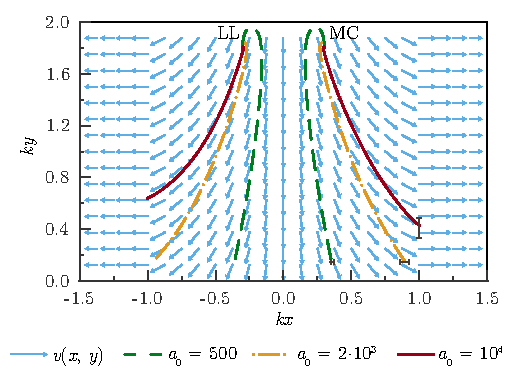
\includegraphics[width=115mm]{asym-betafield}}
%     \caption[\fixme{Динамика электрона около магнитного узла}]{\label{fig:ch1/sec3/betafield}Поле скорости~\eqref{eq:ch1/sec2/rfdv} (стрелки) и траектории электрона в поле~\eqref{eq:ch1/sec3/const_E_lin_B} для различных значений амплитуды поля: $a_0 = 500$
%     (пунктирные линии), $a_0 = 2 \cdot 10^3$ (штрих-пунктирные линии) и $a_0 = 10^4$ (сплошные линии). Электроны стартуют из точки $x_0 = \pm 0.3$ с Лоренц-фактором $\gamma_0 = 100$ и импульсом вдоль оси $y$. Траектории с $x < 0$ вычислены с учётом силы радиационного трения в форме Ландау--Лифшица, траектории с $x > 0$~---~с помощью метода Монте Карло. Планки погрешностей отмечают стандартное отклонение ($\pm \sigma$) от конечного положения электрона, вычисленное по 400 траекториям. Координаты нормированы на $1/k = \lambda / 2 \pi$,
%     где $\lambda = 1$ мкм.}
% \end{figure}


\section{Cвойства и примеры асимптотических траекторий}
\label{sec:ch1/sec4/Properties}
Рассмотрим уравнения~\eqref{eq:ch1/sec2/rfdr} и \eqref{eq:ch1/sec2/rfdv} и исследуем общие свойства траекторий, основываясь на известной симметрии уравнений Максвелла. Следующее преобразование:
\begin{align}
    \label{eq:ch1/sec3/symmetry_t}
    t' &= - t, \\
    \label{eq:ch1/sec3/symmetry_E}
    \vb{E}' &= -\vb{E}, \\
    \label{eq:ch1/sec3/symmetry_B}
    \vb{B}' &= \vb{B}, \\
    \label{eq:ch1/sec3/symmetry_rho}
    \rho' &= -\rho, \\
    \label{eq:ch1/sec3/symmetry_j}
    \vb{j}' &= \vb{j}.
\end{align}
не изменяет уравнения Максвелла в том смысле, что оно приводит к таким же уравнениям для штрихованных переменных. Дальше будем обозначать величины $\vb{E}$, $\vb{B}$, $\vb{j}$, изменяющиеся со временем $t$, \textit{начальной} системой, $\vb{E}'$, $\vb{B}'$, $\vb{j}'$, изменяющиеся со временем $t'$, \textit{штрихованной} системой. Приведённая выше симметрия~---~это соотношение между системой токов, излучающих некоторые поля, и системой токов, поглощающих поля. Данное соотношение заключается в том, что вектор Пойнтинга, скалярное произведение $\vb{j \cdot E}$ и направление времени в штрихованной системе противоположны таковым в начальной системе.
Согласно уравнению~\eqref{eq:ch1/sec2/rfdv}, в штрихованной системе поле скорости $\vb{v}'$ соотносится с полем скорости в начальной системе $\vb{v}$ следующим образом:
\begin{equation}
    \label{eq:ch1/sec3/symmetry_v}
    \vb{v}'(\vb{r}, t') = -\vb{v}(\vb{r}, -t'),
\end{equation}
То есть в штрихованной системе поле скорости и направление времени противоположны таковым в начальной системе, что приводит к траекториям в штрихованной системе $\vb{r}'(t')$ таким же, как и в начальной системе, но проходимым электроном в обратном направлении:
$\dd \vb{r}' / \dd t' = \vb{v}'(\vb{r}', t') = -\vb{v}(\vb{r}', -t')$.
Отметим фундаментальную разницу между асимптотической траекторией, описываемой уравнениями~\eqref{eq:ch1/sec2/rfdv}--\eqref{eq:ch1/sec2/rfdr}, и пондеромоторным описанием. Пондеромоторная сила определяется распределением величин $E^2$ и $B^2$ и соответственно инвариантна относительно преобразования~\eqref{eq:ch1/sec3/symmetry_t}--\eqref{eq:ch1/sec3/symmetry_j}, в то время как это преобразование обращает направление движения электрона, описываемое уравнениями~\eqref{eq:ch1/sec2/rfdv} и \eqref{eq:ch1/sec2/rfdr}, справедливыми при сильной реакции излучения.

Продемонстрируем отличие пондеромоторного и асимптотического описания на следующем примере. Рассмотрим рассеяние электрона двумя лазерными импульсами, распространяющимися навстречу друг другу, расположенными изначально на некотором удалении друг от друга. Пусть первый импульс распространяется вдоль оси $x$, а второй получается из первого преобразованием~\eqref{eq:ch1/sec3/symmetry_t}--\eqref{eq:ch1/sec3/symmetry_B} и соответственно распространяется против оси $x$. Пусть электрон находится ближе к первому импульсу. Тогда, согласно пондеромоторному описанию, первый импульс рассеивает электрон в сторону. В таком случае электрон может оказаться вдали от обоих импульсов и второй импульс вообще не окажет влияние на движение электрона. Однако, если электрон обильно излучает, то справедливо асимптотическое описание его движения. В таком случае траектория электрона в поле второго импульса такая же, как и в поле первого, но проходится в обратном направлении. Поэтому в режиме сильных радиационных потерь электрон после движения в поле первого импульса возвращается на своё изначальное положение, двигаясь в поле второго импульса. Такое поведение крайне отличается от поведения согласно пондеромоторному описанию.

Таким образом, асимптотическое описание подразумевает, что электроны не рассеиваются, а долгое время остаются в поле лазерного пучка. Это заключение находится в хорошем согласии с результатами теоретических соображений и численного моделирования, которые показывают, что пондеромоторная сила может быть значительно подавлена реакцией излучения~\cite{Fedotov14b, Ji14b}.

\subsection{Асимптотические траектории в стоячих волнах}
\label{sub:ch1/sec3/standing-waves}

В данном разделе мы покажем, что уравнения~\eqref{eq:ch1/sec2/rfdr} и \eqref{eq:ch1/sec2/rfdv} всегда приводят к периодическим траекториям в широком классе полей, которые в общем случае записываются в следующем виде:
\begin{eqnarray}
    \label{eq:ch1/sec3/Esw}
    \vb{E} = \vb{f}(\vb{r}, t) - \vb{f}(\vb{r}, -t), \\
    \label{eq:ch1/sec3/Bsw}
    \vb{B} = \vb{g}(\vb{r}, t) + \vb{g}(\vb{r}, -t),
\end{eqnarray}
где $\vb{E = f}(\vb{r}, t)$, $\vb{B = g}(\vb{r}, t)$~---~решения уравнений Максвелла для плотности заряда $\rho$ и плотности тока $\vb{j}$ (для простоты будем рассматривать случай $\rho = 0$ и $\vb{j} = 0$). 
Такое представление обозначает, что поля представляют собой сумму полей в какой то системе и полей в соответствующей штрихованной системе. В таком случае преобразование~\eqref{eq:ch1/sec3/symmetry_t}--\eqref{eq:ch1/sec3/symmetry_j} приводит к таким же полям в штрихованной системе, что и в начальной системе, т.е. $\vb{E}'(\vb{r}, t') = \vb{E}(\vb{r}, t')$, $\vb{B}'(\vb{r}, t')
= \vb{B}(\vb{r}, t')$, что приводит к такому же полю скоростей $\vb{v}'(\vb{r}, t') = \vb{v}(\vb{r}, t')$. С учётом выражения~\eqref{eq:ch1/sec3/symmetry_v} мы имеем:
\begin{equation}
    \vb{v}(\vb{r}, -t) = -\vb{v}(\vb{r}, t),
\end{equation}
т.е. поле скорости в полях~\eqref{eq:ch1/sec3/Esw}--\eqref{eq:ch1/sec3/Bsw}~---~нечётная функция времени. Если помимо прочего поля~\eqref{eq:ch1/sec3/Esw}--\eqref{eq:ch1/sec3/Bsw} являются периодическими функциями времени, то поле скорости также периодично во времени с тем же периодом, $T$. Поэтому среднее по периоду значение скорости равно нулю:
\begin{equation}
    \langle\vb{v}\rangle_T=\int_0^{T} \vb{v}(t')\,dt'=\int_{-T}^{0}\vb{v}(-t')\,dt'=-\int_{0}^{T}\vb{v}(t')\,dt'=-\langle\vb{v}\rangle_T.
\end{equation}
В связи с этим
\begin{equation}
    \vb{r}(t+T)=\int_0^{t+T} \vb{v}(t')\,dt'=\int_0^t \vb{v}(t')\,dt'+\int_t^{t+T} \vb{v}(t')\,dt'=\vb{r}(t)+\langle\vb{v}\rangle_T=\vb{r}(t).
\end{equation}
Таким образом, в периодических полях~\eqref{eq:ch1/sec3/Esw}--\eqref{eq:ch1/sec3/Bsw} в рамках асимптотического описания, электрон периодически движется по одному и тому же пути.

Ниже рассмотрим несколько конкретных примеров конфигураций стоячих волн, в которых сравним асимптотические траектории и численное решение неукороченных уравнений движения.

\subsection{Асимптотические траектории в линейно-поляризованной стоячей волне}
Конфигурация полей в стоячей линейно-поляризованной достаточно проста, поэтому асимптотические траектории можно найти в явном виде.
Пусть $\vb E = \vb{y_0} \cos (t) \cos (x)$, $\vb B = \vb{z_0} \sin (t) \sin (x)$, тогда
\begin{equation}
    \vb v = \begin{cases}
    \vb{x_0} \tg (t) \tg (x) + \vb{y_0} \sqrt{1-\tg^2(t) \tg^2(x)},&\text{если $E>B$;}\\
    \vb{x_0} \ctg (t) \ctg (x),&\text{если $E<B$.}
    \end{cases}
\end{equation}
Так как поля однородны вдоль оси $y$, то движение вдоль неё не представляет большого интереса. Зависимость $x(t)$ определяется из уравнений:
\begin{equation}
\label{fig:ch1/sec3/xt_lpw}
    \begin{cases}
        \sin (x) \cos(t) = \sin (x_0) \cos (t_0),&\text{если $E>B;$}\\
        \cos (x) \sin(t) = \cos (x_0) \sin (t_0),&\text{если $E<B.$}
    \end{cases}
\end{equation}
Пусть электрон в момент времени $t=0$ находится в точке $x=x_0$ такой, что $E>B$ (иначе электрон будет покоится до момента, пока не будет выполнено это условие). Траектория электрона определяется первым уравнением в (\ref{fig:ch1/sec3/xt_lpw}), пока он не дойдёт до точки, в которой $E=B$; после этого траектория определяется вторым уравнением в (\ref{fig:ch1/sec3/xt_lpw}) вплоть до следующей точки, в которой выполняется условие $E=B$ и так далее. 
Такие точки определяются из условия $\tg(x)\tg(t)=1$. Отсюда можно явно найти точку изменения траектории, до которой дойдёт электрон, стартуя в момент $t=0$ из точки $x_0$:
\begin{equation}
    \ctg x_1 = \tg t_1 = \sqrt{\frac{1}{\sin (x_0)} - 1}
\end{equation}
Легко показать, что электрон достигнет следующей ближайшей точки изменения траектории в момент времени $t_2 = \pi - t_1$ с координатой $x_2 = x_1$, а следующей в $t_3 = \pi + t_1$ с координатой $x_3 = x_1$ и дальше траектория будет периодически повторяться.
Траектории электронов, стартующих из других точек, находятся аналогичным образом.
Явный вид траекторий $x(t)$ и их сравнение с численным решением неукороченных уравнений движения представлены на Рис.~\ref{fig:ch1/sec3/onion}.
Согласно рассуждениям в п.~\ref{sub:ch1/sec3/standing-waves}, асимптотические траектории электрона в стоячей линейно-поляризованной волне являются периодическими.
Однако известно, что поведение электронов в сильной стоячей волне сопровождается так называемым~\textit{аномальным радиационным захватом}~\cite{Gonoskov14}~---~приближением частиц к узлу магнитного поля, который является неустойчивым положением равновесия без учёта реакции излучения.
Аномальный радиационный захват вызван дрейфом электрона между различными асимптотическими траекториями~\eqref{fig:ch1/sec3/xt_lpw}, который занимает много периодов поля~\cite{Gonoskov14} и поэтому не описывается представленной асимптотической теорией.
Отметим, что в случае $a_0 = 10^5$ траектории электронов, вычисленные с помощью метода Монте-Карло, приближаются к узлу магнитного поля с каждым следующим периодом, что и является аномальным радиационным захватом (см. Рис.~\ref{fig:ch1/sec3/onion}).

\begin{figure}[ht]
    \centerfloat{\includegraphics{asym-onion}}
    \caption[Динамика электрона в линейно-поляризованной стоячей электромагнитной волне]{Динамика электрона в линейно-поляризованной стоячей электромагнитной волне. (a) Сплошные серые линии~---~асимптотические траектории, вычисленные по уравнению~\eqref{eq:ch1/sec2/rfdr}. Области преобладания электрического и магнитного поля отмечены светло оранжевым и светло зелёным цветами соответственно. Сплошные цветные линии~---~численные траектории, вычисленные по классическим уравнениям движения с учётом квантовой реакции излучения с помощью метода Монте-Карло (см. Приложение~\ref{app:numerical}) для $a_0 = 10^3$ и $a_0 = 10^5$ (стартующие из $x < 0$ и $x > 0$ соответственно). Штриховые оранжевые линии соответствуют магнитному узлу стоячей волны ($B = 0$), штрих-пунктирные зелёные линии~---~электрическому узлу стоячей волны ($E=0$).
    (b) Энергия частицы как функция времени для численных траекторий, нормированная на величину $a_0$.}
    \label{fig:ch1/sec3/onion}
\end{figure}

\subsection{Асимптотические траектории в лазерном пучке конечного диаметра}
\label{sub:ch1/TE11}

\begin{figure}[ht]
    \centerfloat{\includegraphics{te11-new}}
    \caption[Динамика электрона в поле ТЕ11 моды прямоугольного волновода]{\label{fig:ch1/sec3/te11}
    (a) Электрическое и магнитное поля (зелёные и синие стрелки соответственно) ТЕ11 моды волновода~\eqref{eq:ch1/sec3/te11-1}--\eqref{eq:ch1/sec3/te11-6} при t = 0.
    (b) Асимптотические траектории, вычисленные по уравнениям~\eqref{eq:ch1/sec2/rfdr}, \eqref{eq:ch1/sec2/eta_explicit} и
    \eqref{eq:ch1/sec2/betaB}--\eqref{eq:ch1/sec2/betaEEB} в лабораторной системе отсчёта; $\xi = x - v_g t$, где
    $v_g$~---~групповая скорость TE11 моды.
    (c) Та же асимптотическая траектория (синяя линия) и траектории электронов, рассчитанные численно (см. Приложение~\ref{app:numerical}), стартующих из точки $x = 0$, $y = 0.2 \, \lambda$, $z = 0.65 \, \lambda$ ($\lambda = 1$ мкм, $t \in [0, 2 \tau]$), для $a_0 = 700$ (зелёная линия) и $a_0 = 4 \cdot 10^3$ (красная линия).}
\end{figure}

Покажем, что большое число конфигураций электромагнитного поля может быть представлено в виде периодических полей обладающих <<излучательно-поглощательной>> симметрией~\eqref{eq:ch1/sec3/symmetry_t}--\eqref{eq:ch1/sec3/symmetry_j}. Также мы представим один из способов разрешения неоднозначности поля скорости, задаваемого уравнением~\eqref{eq:ch1/sec2/eta_explicit}.

Рассмотрим поля ТЕ11 моды в прямоугольном металлическом волноводе:
\begin{eqnarray}
    \label{eq:ch1/sec3/te11-1}
    E_x = 0, \\
    \label{eq:ch1/sec3/te11-2}
    E_y = a_0 \cos(k_y y) \sin(k_z z) \cos(t - k_x x), \\
    \label{eq:ch1/sec3/te11-3}
    E_z = -\frac{a_0 k_y}{k_z} \sin(k_y y) \cos(k_z z) \cos(t - k_x x), \\
    \label{eq:ch1/sec3/te11-4}
    B_x = \frac{a_0 (k_z^2 + k_y^2)}{k_z} \cos(k_y y) \cos(k_z z) \sin(t - k_x x), \\
    \label{eq:ch1/sec3/te11-5}
    B_y = -k_x E_z, \\
    \label{eq:ch1/sec3/te11-6}
    B_z = k_x E_y,
\end{eqnarray}
где угловая частота волны $\Omega = (k_x^2 + k_y^2 + k_z^2)^{1/2}= 1$ (мы используем нормировочную частоту $\omega$ равную частоте волны и, как раньше, время нормировано на $1/\omega$, координаты~---~на $c / \omega$, $\vb k$~---~волновое число, нормированное на $\omega / c$).
Данные поля имеют металлические граничные условия при ${y = 0, \; \pm \ell_y, \; \pm 2 \ell_y,...}$ ($E_z = 0$) и при ${z = 0, \; \pm \ell_z, \; \pm 2 \ell_z,...}$ ($E_y = 0$), где $\ell_y = \pi / k_y$ и $\ell_z = \pi / k_z$~---~размеры волновода вдоль осей $y$ и $z$ соответственно.

Поля~\eqref{eq:ch1/sec3/te11-1}--\eqref{eq:ch1/sec3/te11-6} являются решениями уравнения Максвелла не только внутри волновода, но и в вакууме, т.к. они могут быть представлены в виде суммы плоских волн. Будем рассматривать эти поля в области ${y \in [-\ell_y / 2, \ell_y /2]}$ и $z \in [0, \ell_z]$ в качестве модели лазерного пучка конечного диаметра.
Асимптотическая траектория в таких полях представлена на Рис.~\ref{fig:ch1/sec3/te11} (а), где $\xi = x - v_g t$, $v_g=k_x$~---~групповая скорость ТЕ11 моды. Траектория начинается при $t = 0$ в точке $x = 0$, $y = 0.2$, $z = 0.65$ и заканчивается при $t = 2 \tau$, где $\tau$~---~характерный временной масштаб задачи:
\begin{equation}
    \label{tau}
    \tau = \frac{2 \pi}{k_x (v_\varphi - v_g)} = \frac{2 \pi}{1 - k_x^2}
\end{equation}
где $v_\varphi = 1 / v_g$~---~фазовая скорость волны. 

Из Рис.~\ref{fig:ch1/sec3/te11} видно, что асимптотическая траектория квазипериодическая, что достаточно хорошо согласуется с траекторией реального электрона при $a_0= 4 \cdot 10^3$, который долгое время остаётся в области сильного поля. Однако, как будет показано ниже, вдоль асимптотических траекторий, вычисленных в лабораторной системе отсчёта, значения $\xi$ и период траектории плохо совпадают с таковыми для реальных траекторий электрона. Это связано с тем, что выражение~\eqref{eq:ch1/sec2/eta_explicit} не является Лоренц-инвариантом, поэтому вычислив скорость $\vb v$ с помощью этого выражения в одной системе отсчёта, в какой-то другой системе отсчёта, мы получим ${\vb v}' = \vb{E}' \times \vb{B}' + a \vb{B}'$, где $a$~---~константа.

Рассмотрим поля~\eqref{eq:ch1/sec3/te11-1}--\eqref{eq:ch1/sec3/te11-6} в системе отсчёта $K'$, движущейся вдоль оси $x$ с груповой скоростью $v_g$:
\begin{eqnarray}
    \label{eq:ch1/sec3/te11'-1}
    E_y' = a_0 k_\perp \cos(k_y y) \sin(k_z z) \cos(k_\perp t'), \\
    \label{eq:ch1/sec3/te11'-2}
    E_z' = -\frac{a_0 k_\perp k_y}{k_z} \sin(k_y y) \cos(k_z z) \cos(k_\perp t'), \\
    \label{eq:ch1/sec3/te11'-3}
    B_x' = \frac{a_0 (k_z^2 + k_y^2)}{k_z} \cos(k_y y) \cos(k_z z) \sin(k_\perp t'), \\
    \label{eq:ch1/sec3/te11'-4}
    E_x' = B_x' = B_y' = B_z' = 0,
\end{eqnarray}
где $k_\perp = \sqrt{1 - k_x^2}$. Эти поля не зависят от $x'$ и для всех электронов а таком поле компонента силы Лоренца вдоль оси $x'$ отсутствует. Более того, из-за радиационных потерь электроны <<забывают>> своё начальное направление движения, поэтому мы будем полагать, что в полях~\eqref{eq:ch1/sec3/te11'-1}--\eqref{eq:ch1/sec3/te11'-4} средняя скорость электронов $v_x' = 0$. Поэтому в лабораторной системе отсчёта $K$ средняя скорость электронов $v_x = v_g$ и следовательно $\xi = \operatorname{const}$. Отметим, что это утверждение неверно для асимптотических траекторий, вычисленных в лабораторной системе отсчёта (см. Рис.~\ref{fig:ch1/sec3/te11} (a)), что в частности приводит к отличному значению периода $y$ и $z$ координат.

Замены $t' \rightarrow t' + \pi / 2 k_\perp$ и $t' \rightarrow -t'$ указывают на то, что электрические поля~\eqref{eq:ch1/sec3/te11'-1}--\eqref{eq:ch1/sec3/te11'-2} являются нечётными функциями времени, а магнитные~\eqref{eq:ch1/sec3/te11'-3}~---~чётными в $K'$ и все поля являются периодическими. В соответствии с разделом~\ref{sub:ch1/sec3/standing-waves} в таком случае в рамках асимптотического описания траектории электронов также периодические с периодом $2 \pi / k_\perp$ в $K'$. В таком случае в лабораторной системе отсчёта электроны движутся вдоль оси $x$ с групповой скоростью лазера и, т.к. $y' = y$ и $z' = z$, траектории электрона периодические в плоскости $yz$ с периодом
\begin{equation}
    T = \frac{2 \pi}{k_\perp \sqrt{1 - v_g^2}} = \tau.
\end{equation}
Таким образом, неоднозначность поля скорости в асимптотическом подходе может быть разрешена выбором правильной системы отсчёта.

Итак, мы показали, что асимптотическое описание~\eqref{eq:ch1/sec2/rfdr} и \eqref{eq:ch1/sec2/rfdv} приводит к периодическим траекториям в широком классе стоячих волн (например, сформированных лазерными пучками конечного диаметра) и движению электронов вдоль оси распространения лазерного импульса с его групповой скоростью и периодическим поперечным движением.
Последнее может объяснять эффект захвата частиц за счёт реакции излучения~\cite{Ji14b}.


\section{Поправки к асимптотической теории}
\label{sec:ch1/sec4}

Разработанная выше теория позволяет описывать динамику электрона в условиях экстремальных радиационных потерь без уточнения конкретного вида мощности последних, и таким образом представляет собой полезный аналитический инструмент, с помощью которого нами были получены некоторые новые результаты.
Однако, такой подход обладает двумя существенными ограничениями.
Во-первых, как показано выше настоящие траектории электрона сходятся к асимптотическим достаточно быстро только при экстремальных интенсивностях, превышающих $\SI{e25}{\watt/\centi\meter^2}$ (при длине волны $\lambda=\SI{1}{\um}$).
Это связано с тем, что для большинства реалистичных конфигураций ЭМ поля характерное время, за которое вектор скорости электрона приближается к безрадиационному направлению, недооценивается в наших рассуждениях, приведённых фактически для постоянного ЭМ поля.
Во-вторых, с помощью разработанного нами подхода оказывается невозможным вычислить энергию и радиационные потери электрона, при приближении к асимптотической траектории, т.к. энергия электрона предполагается неограниченно большой, хотя при этом и много меньшей безразмерной амплитуды ЭМ поля.
Несмотря на указанные недостатки, схожий подход был недавно успешно применён для описания динамики электронов в некоторых астрофизических задачах~\cite{jerome2022particle}.

Для избавления от указанных выше недостатков построим теорию возмущений, предположив, что скорость электрона отклоняется от безрадиационного направления, но это отклонение мало, т.е. представим скорость электрона в следующем виде
\begin{equation}
    \vb{v}=\left( 1 - \frac{\delta^2}{2} \right) \vb{v}_0 + \vb{v}_1,
\end{equation}
где $\vb{v}_1\perp\vb{v}_0$ и $\delta$ могут быть найдены из связи с энергией электрона ${|\vb{v}|^2= 1-\gamma^{-2}}$ следующим образом
\begin{equation}
    \delta^2\approx v_1^2+\gamma^{-2}.
\end{equation}
% 
% \begin{gather}
%     \dv{\vb{v}}{t} = -\frac{1}{\gamma} \left( \vb{E} + \vb{v}\times\vb{B} - \vb{v} (\vb{v}\vb{E}) \right) = -\frac{\vb{F}_\perp}{\gamma} \\
%     \dv{\gamma}{t} = -\vb{v}{E} - F_\mathrm{rr} v^2
% \end{gather}
% 
Подставим данное представление скорости в уравнение~\eqref{eq:ch1/sec2/base2} и разложим его до слагаемых не выше второго порядка по $\delta$. 
Отдельно рассмотрим слагаемое $\vb{F}_\perp$ в правой части получившегося уравнения:
\begin{equation}
    \begin{multlined}[t]
        \vb{F}_\perp = -\frac{\delta^2}{2} [\vb{v}_0 \times \vb{B}] + [\vb{v}_1 \times \vb{B}]  + \delta^2 \vb{v}_0(\vb{v}_0 \vb{E}) - \vb{v}_0(\vb{v}_1 \vb{E}) - \vb{v}_1(\vb{v}_0 \vb{E}) - \vb{v}_1(\vb{v}_1 \vb{E}) + \mathcal{O}(\delta^3)
    \end{multlined}
\end{equation}
Рассмотрим отдельно выражение $\vb{v}_1 \times \vb{B}$:
\begin{equation}
    \label{eq:ch1/sec4/v1b}
    \begin{aligned}
         & \vb{v}_1 \times \vb{B} = -(\vb{v}_0 \vb{B})[\vb{v}_0 \times \vb{v}_1] + \vb{v}_0 (\vb{v}_0[\vb{v}_1\times \vb{B}]).
    \end{aligned}
\end{equation}
Произведём скалярное умножение уравнения~\eqref{eq:ch1/sec2/rfd1} на $\vb{v}_1$
\begin{equation}
    (\vb{v}_1 \vb{E}) + \vb{v}_1 [\vb{v}_0\times \vb{B}] = 0.
\end{equation}
Выполнив циклическую перестановку в смешанном произведении, получим
\begin{equation}
    \label{eq:ch1/sec4/v0v1B}
    \vb{v}_0 [\vb{v}_1\times \vb{B}] = (\vb{v}_1 \vb{E}).
\end{equation}
Таким образом,
\begin{equation}
    \vb{v}_1 \times \vb{B} = \vb{v}_0 (\vb{v}_1 \vb{E}) - [\vb{v}_0 \times \vb{v}_1] (\vb{v}_0 \vb{B})
\end{equation}
Выполняя аналогичные действия, можно записать слагаемое $\vb{v}_0 \times \vb{B}$ в следующем виде:
\begin{equation}
    \vb{v}_0 \times \vb{B} = -\vb{v}_1 \frac{(\vb{v}_1 \vb{E})}{v_1^2} + [\vb{v}_0\times\vb{v}_1] \frac{(\vb{v}_1 \vb{B})}{v_1^2}
\end{equation}
Таким образом поперечная сила $\vb{F}_\perp$ может быть записана в виде разложения в ортогональном базисе $\vb{v}_0$, $\vb{v}_1$, $\vb{v}_0\times\vb{v}_1$ следующим образом
\begin{equation}
    \label{eq:ch1/sec4/fperp}
    \begin{aligned}
        \vb{F}_\perp = &\,\vb{v}_0 (\vb{v}_0 \vb{E}) \delta^2 -\\
                     - &\,\vb{v}_1 \left( (\vb{v}_0 \vb{E}) + (\vb{v}_1 \vb{E})\frac{v_1^2 - \gamma^{-2} }{2v_1^2} \right) -\\
                     - &\,[\vb{v}_0\times\vb{v}_1] \left( (\vb{v}_0 \vb{B}) + (\vb{v}_1 \vb{B}) \frac{v_1^2 + \gamma^{-2}}{2v_1^2}\right) .
    \end{aligned}
\end{equation}
Рассмотрим левую часть уравнения~\eqref{eq:ch1/sec2/base2}
\begin{equation}
    \label{eq:ch1/sec4/2nd_order_A}
    \dv{\vb{v}}{t} = \left( 1 - \frac{\delta^2}{2} \right)\dv{\vb{v}_0}{t} - \frac{\vb{v}_0}{2}\left( \dv{v_1^2}{t}+ \dv{\gamma^{-2}}{t} \right) + \dv{\vb{v}_1}{t} 
\end{equation}
Для вычисления слагаемого $\dd v_1^2/\dd t$ умножим скалярно уравнение~\eqref{eq:ch1/sec2/base2} на $\vb{v}_1$, учитывая, что $\vb{v}_1 \vb{v}_0=0$, и отбрасывая слагаемые высших порядков малости
\begin{equation}
    \frac{1}{2} \dv{v_1^2}{t} = - \vb{v}_1\dv{\vb{v}_0}{t} + \frac{v_1^2(\vb{v}_0 \vb{E})}{\gamma}.
\end{equation}
Разложим слагаемое, содержащее $\dd \gamma^{-2} /\dd t$, воспользовавшись уравнением~\eqref{eq:ch1/sec2/base2}:
\begin{align}
    \label{eq:ch1/sec4/dg2dt}
    \frac{1}{2}\dv{\gamma^{-2}}{t} = -\frac{1}{\gamma^3}\dv{\gamma}{t} \approx \frac{\vb{v}_0\vb{E} }{\gamma^3}
\end{align}
Таким образом,
\begin{equation}
    \label{eq:ch1/sec4/ddeltadt}
    \frac{1}{2}\dv{\delta^2}{t} = - \vb{v}_1\dv{\vb{v}_0}{t} + \delta^2 \frac{(\vb{v}_0 \vb{E})}{\gamma}.
\end{equation}
Подставляя выражения~\eqref{eq:ch1/sec4/ddeltadt} и~\eqref{eq:ch1/sec4/fperp} обратно в уравнение~\eqref{eq:ch1/sec2/base2}, получим
\begin{gather}
    \label{eq:ch1/sec4/2nd_order_B}
    \dv{\vb{v}_1}{t} = \frac{\vb{F}_1}{\gamma} - \left( 1 - \frac{\delta^2}{2} \right)\dv{\vb{v}_0}{t} -\vb{v}_0\left(\vb{v}_1\dv{\vb{v}_0}{t} \right), \\
    \label{eq:ch1/sec4/f1_A}
    \vb{F}_1 = \vb{v}_1 \left( (\vb{v}_0 \vb{E}) + (\vb{v}_1 \vb{E})\frac{v_1^2 - \gamma^{-2} }{2v_1^2} \right)
    + [\vb{v}_0\times\vb{v}_1] \left( (\vb{v}_0 \vb{B}) + (\vb{v}_1 \vb{B}) \frac{\delta^2}{2v_1^2}\right) .
\end{gather}
Наконец, найдём выражение для КЭД параметра $\chi$, исходя из его определения~\eqref{eq:ch1/sec1/chi} и проведённых выше вычислений
\begin{equation}
    \chi = \frac{\gamma \delta}{a_\mathrm{S}}\sqrt{\left[ \left( \vb{v}_0 \vb{E} \right)^2 + \left( \vb{v}_0\vb{E} \right)\left( \vb{v}_1\vb{E} \right) + \left( \vb{v}_0\vb{B} \right)\left( \vb{v}_1\vb{B} \right) \right] + \frac{\delta^2}{4v_1^2}\left[ \left( \vb{v}_1 \vb{E} \right)^2 + \left( \vb{v}_1 \vb{B} \right)^2 \right]}
\end{equation}

В итоге мы получили следующую систему общих уравнений, описывающих динамику электрона в условиях экстремальных радиационных потерь
\begin{gather}
    \label{eq:ch1/main1}
    \dv{\vb{v}_1}{t} = \frac{\vb{F}_1}{\gamma} - \left( 1 - \frac{\delta^2}{2} \right)\dv{\vb{v}_0}{t} -\vb{v}_0\left(\vb{v}_1\dv{\vb{v}_0}{t} \right), \\
    \label{eq:ch1/main2}
    \dv{\gamma}{t} = -\vb{v}_0\vb{ E} \left( 1 - \frac{\delta^2}{2} \right) - \vb{v}_1 \vb{E} - F_\mathrm{rr}(\chi) ,                                                                       \\
    \label{eq:ch1/f1}
    \vb{F}_1 = \vb{v}_1 \left( (\vb{v}_0 \vb{E}) + (\vb{v}_1 \vb{E})\frac{v_1^2 - \gamma^{-2} }{2v_1^2} \right)
    + [\vb{v}_0\times\vb{v}_1] \left( (\vb{v}_0 \vb{B}) + (\vb{v}_1 \vb{B}) \frac{\delta^2}{2v_1^2}\right) , \\
    \label{eq:ch1/base_chi}
    \chi = \frac{\gamma \delta}{a_\mathrm{S}}\sqrt{\left[ \left( \vb{v}_0 \vb{E} \right)^2 + \left( \vb{v}_0\vb{E} \right)\left( \vb{v}_1\vb{E} \right) + \left( \vb{v}_0\vb{B} \right)\left( \vb{v}_1\vb{B} \right) \right] + \frac{\delta^2}{4v_1^2}\left[ \left( \vb{v}_1 \vb{E} \right)^2 + \left( \vb{v}_1 \vb{B} \right)^2 \right]}.
\end{gather}
Отметим, что несмотря на то, что величина $\chi$ пропорциональна малому параметру $\delta$, она может быть произвольно большой за счёт множителя $\gamma$.
В связи с этим слагаемое $F_\mathrm{rr}$ должно быть сохранено во всех порядках разложения, что приводит к тому, что укороченные уравнения движения остаются нелинейными.
% Данное замечание не противоречит тому факту, что последнее слагаемое в уравнении~\eqref{eq:ch1/sec2/base2} намного меньше суммы первых трёх, равной $\vb{F}_\perp$, и потому было опущено в самом начале анализа.
% Действительно, ${|F_\mathrm{rr} \vb{v} / \gamma^2|\lesssim \alpha a_\mathrm{S} \chi^2 / \gamma^2 \approx \alpha |\vb{F}_\perp|^2 / a_\mathrm{S} \sim  \alpha E v_1 |\vb{F}_\perp| / a_\mathrm{S}  \lll |\vb{F}_\perp|}$, в силу того, что $E \ll a_\mathrm{S}$, $\alpha \ll 1$, $v_1 \lesssim 1$.
Также важно отметить, что полные производные в уравнениях выше должны пониматься в смысле производной векторного поля $\vb{v}_0$ вдоль траектории частицы $\vb{r}(t)$, т.е.
\begin{equation}
    \dv{\vb{v}_0}{t} = \pdv{\vb{v}_0}{t} + (\vb{v},\nabla)\vb{v}_0 .
\end{equation}
Рассмотрим уравнение на малый параметр $\delta^2$
\begin{equation}
    \label{eq:ch1/dv2dt}
    \frac{1}{2}\dv{\delta^2}{t} = - \vb{v}_1\dv{\vb{v}_0}{t} + \frac{\delta^2(\vb{v}_0 \vb{E})}{\gamma}.
\end{equation}
Из этого уравнения можно оценить характерное время приближения траектории электрона к асимптотической безрадиационной траектории в постоянном ЭМ поле ($\dd\vb{v}_0/\dd t = 0$)
\begin{equation}
    \tau_v = \frac{\gamma}{|\vb{v}_0 \vb{E}|} \sim \frac{\gamma}{a_0}.
\end{equation}
Однако, для ЭМ поля общего вида знак первого слагаемого в уравнении~\eqref{eq:ch1/dv2dt} может быть произвольным, а его величина сравнимой с $v_1$, поэтому одного условия $\gamma \ll a_0$ недостаточно для того, чтобы оправдать асимптотическое описание динамики электрона в нулевом порядке~\eqref{eq:ch1/sec2/rfdr} в произвольном ЭМ поле.
Таким образом, необходимо использовать именно систему уравнений~\eqref{eq:ch1/main1}--\eqref{eq:ch1/main2}, в которых учитывается отклонение вектора скорости от безрадиационного направления.
Кроме того, с помощью данных уравнений можно найти энергию электрона и его радиационные потери при движении в ЭМ поле.

Приведём объяснение процедуры, произведённой для получения укороченных уравнений движения, с помощью простых шагов.
Во-первых, было показано, что существует некое выделенное безрадиационное направление, к которому в постоянном ЭМ поле стремится вектор скорости электрона.
Раскладывая вектор скорости в базисе, в котором одна ось совпадает с безрадиационным направлением, можно разбить уравнения движения электрона на две составляющие.
Движение вдоль безрадиационного направления фактически описывается энергией частицы, тогда как уравнения на поперечную скорость могут быть разложены в ряд, который очевидно сходится, т.к. длина вектора скорости электрона строго меньше единицы.
Несмотря на то, что полученная система укороченных уравнений остаётся нелинейной и не допускает решения в общем виде, ниже будет рассмотрены примеры, которые показывают, что данный подход может быть более продуктивным, чем решение неукороченных уравнений движения.
Отметим также, что недавно в публикации~\cite{cai2022dynamics} было использовано похожее разложение для нахождения равновесных решений уравнений~\eqref{eq:ch1/main1}--\eqref{eq:ch1/main2}.

Рассмотрим далее конкретные примеры конфигураций ЭМ поля, в которых уравнения~\eqref{eq:ch1/main1}--\eqref{eq:ch1/main2} в том или ином виде могут быть явно разрешены.

\subsection{Обобщённая задача Зельдовича}
\label{sub:ch1/sec4/Zeldovich}

Уравнения движения электрона с учётом реакции излучения могут быть аналитически решены в однородном вращающемся электрическом поле, что было впервые продемонстрировано Я.~Б.~Зельдовичем~\cite{Zeldovich75}. 
Недавно в публикации~\cite{Kostyukov2016} решение Зельдовича было расширено на случай, когда помимо электрического поля присутствует параллельное ему однородное магнитное поле, вращающееся с той же частотой.
Данная конфигурация ЭМ поля вызывает интерес в первую очередь потому, что она, за исключением однородности, образуется при интерференции двух циркулярно-поляризованных волн, распространяющихся навстречу друг другу.
В данной модельной конфигурации поля было построено одно из первых приближённых решений задачи о развитии КЭД каскада~\cite{fedotov2010limitations, elkina2011qed}.
Построим решение задачи о движении электрона в таком ЭМ поле, воспользовавшись разработанной нами теорией.
Предположим, что электрическое и магнитное поля однородны, параллельны и вращаются с угловой частотой $\symbf{\Omega}$.
Безрадиационное направление в таком случае противоположно направлено электрическому полю: ${\vb{v}_0 = -\vb{E}/E \equiv -\vb{e}}$.
Будем интересоваться стационарным решением, при котором вектор скорости электрона синхронно вращается с электрическим и магнитным полем.
В таком случае в уравнении~\eqref{eq:ch1/main1} можно заменить производные по времени на векторное произведение $\symbf{\Omega}\times$
\begin{equation}
    \label{eq:ch1/zeldovich}
    \symbf{\Omega}\times\vb{v}_1 = -\frac{E}{\gamma}\vb{v}_1 + \frac{B}{\gamma}\vb{e\times v}_1 + \symbf{\Omega\times e} + v_1 \vb{e}.
\end{equation}
Используя тот факт, что $\vb{v}_1 \perp \vb{v}_0$, вектор $\vb{v}_1$ можно разложить по компонентам следующим образом
\begin{equation}
    \vb{v}_1 = v_\perp \symbf{\Omega}\times\vb{e} + v_x \symbf{\Omega} .
\end{equation}
В таком случае уравнение~\eqref{eq:ch1/zeldovich} разделяется на систему линейных уравнений, решение которых легко находится
\begin{gather}
    \label{eq:ch1/Zeld_sol1}
    v_x = \frac{\gamma B}{E^2 + B^2} ,\\
    \label{eq:ch1/Zeld_sol2}
    v_\perp = \frac{\gamma E}{E^2 + B^2}, \\
    v_1 = \frac{\gamma}{\sqrt{E^2 + B^2}} .
\end{gather}
Стационарность решения также подразумевает, что набор энергии электроном в электрическом поле точно скомпенсирован радиационными потерями там, что $\dd\gamma/\dd t = 0$.
В таком случае связь между энергией электрона и амплитудой электрического поля находится из следующего уравнения
\begin{gather}
    E \left(1 - \frac{\delta^2}{2}\right) = F_\mathrm{rr}\left(\frac{\gamma\delta E}{a_\mathrm{S}}\right) , \\
    \delta = \sqrt{v_1^2 + \gamma^{-2}} = \sqrt{\frac{\gamma^2}{E^2 + B^2} + \frac{1}{\gamma^2}}.
\end{gather}
Полученный результат в точности совпадает с результатом, полученным в публикации~\cite{Kostyukov2016}, и в частном случае $B=0$~---~с результатом оригинальной статьи~\cite{Zeldovich75}.
\fixme{Добавить классический предел $\chi \ll 1$, $B=0$}
\begin{figure}[ht]
    \centerfloat{\includegraphics{asym-Zeldovich}}
    \caption[Динамика электрона в синхронно вращающихся однородных параллельных электрическом и магнитном полях]{
    Динамика электрона в электрическом поле с безразмерной амплитудой $eE/mc\Omega = \num{2500}$ и параллельном магнитном поле с безразмерной амплитудой $eB/mc\Omega = \num{2000}$, синхронно вращающихся с угловой частотой $\Omega$, соответствующей длине волны $\lambda = 2\pi c /\Omega = \SI{1}{\um}$: (a) компонента скорости электрона поперёк электрического поля в плоскости вращения, (b) компонента скорости электрона вдоль вектора угловой скорости $\symbf{\Omega}$. Зелёные (голубые) линии соответствуют численному решению неукороченных уравнений движения электрона~\eqref{eq:ch1/sec2/base1}--\eqref{eq:ch1/sec2/base2} с учётом реакции излучения с помощью полуклассического (квантового) подхода (см. Приложение~\ref{app:numerical}), синие линии соответствуют величинам, усреднённым по 100 реализациям <<квантовых>> решений. Оранжевые линии соответствуют аналитическому решению~\eqref{eq:ch1/Zeld_sol1}--\eqref{eq:ch1/Zeld_sol2}.}
    \label{fig:ch1/sec5/zeldovich}
\end{figure}
Сравнение полученного решения с результатом численного решения неукороченных уравнений движения~\eqref{eq:ch1/sec2/base1}--\eqref{eq:ch1/sec2/base2} с учётом реакции излучения как с помощью полуклассического, так и квантового подхода, представлено на Рис.~\ref{fig:ch1/sec5/zeldovich}.
Параметры ЭМ поля в данном случае были выбраны таким образом, чтобы среднее значение КЭД параметра $\chi$ электрона составляло около 5.
Данный выбор был осуществлён для демонстрации границ применимости нашего подхода.
В нашей теории, которая основывается на полуклассическом подходе к описанию реакции излучения, предполагается, что величина КЭД параметра $\chi$ существенно не различается в процессе движения для электронов с близкими начальными условиями.
В таком случае можно считать, что усреднённая по функции распределения электронов сила радиационного трения может быть вычислена, как сила трения, действующая на <<средний>> электрон, т.е. $\langle F_\mathrm{rr} (\chi) \rangle \approx F_\mathrm{rr}(\langle\chi\rangle)$, где угловые скобки означают усреднение по функции распределения электронов.
Однако, как видно из Рис.~\ref{fig:ch1/sec5/zeldovich} параметры электронов с одинаковыми начальными условиями, в процессе движения приобретают существенный разброс, связанный со стохастичностью процесса излучения.
В связи с этим и характером зависимости $F_\mathrm{rr}(\chi)$ в существенно квантовом режиме справедливо неравенство $\langle F_\mathrm{rr} (\chi) \rangle < F_\mathrm{rr}(\langle\chi\rangle)$, что объясняет различие между значениями $v_x$ и $v_\perp$, полученными согласно аналитическому решению~\eqref{eq:ch1/Zeld_sol1}--\eqref{eq:ch1/Zeld_sol2} и полученными в результате усреднения по различными реализациям квантовых численных решений, наблюдаемое на Рис.~\ref{fig:ch1/sec5/zeldovich} (b).

\subsection{Плазменный ускоритель}
\label{sub:ch1/sec5/Accelerator}
Рассмотрим <<игрушечную модель>> плазменного ускорителя и найдём известное устойчивое квазистационарное решение в режиме экстремальных радиационных потерь~\cite{kostyukov2012radiative, golovanov2021radiation} с помощью разработанной нами теории.
Для этого будем считать, что ЭМ поле является суммой однородного ускоряющего электрического поля $\vb{z}_0 E_\mathrm{acc}$ и линейно зависящего от поперечных координат фокусирующего электрического поля $\vb{y} E_\mathrm{foc}$, в котором электроны совершают бетатронные колебания.
Чтобы найти решение, которое соответствует постоянству радиационных потерь, усреднённых по периоду бетатронных колебаний, предположим, что произвольная функция КЭД параметра $\chi$ является строго периодической функцией времени, т.е. её среднее является константой.
Математически данное условие записывается следующим образом
\begin{equation}
    \label{eq:ch1/acc_const_av}
    \dv{\langle \chi^2 \rangle}{t} = 0 ,
\end{equation}
где функция $\chi^2$ использована для удобства дальнейших рассуждений.
В рассматриваемой конфигурации ЭМ поля из уравнения~\eqref{eq:ch1/base_chi} легко получить выражение для $\chi$
\begin{equation}
    \label{eq:ch1/sec5/acc/chi}
    \chi = \frac{\gamma \delta E}{a_\mathrm{S}}.
\end{equation}
Здесь и далее будем считать, что выполняется условие $\gamma \approx \langle \gamma \rangle$, т.е. амплитуда колебаний энергии электрона существенно меньше величины самой энергии.
В таком случае энергию $\gamma$ во всех вычислениях можно выносить из под знака усреднения.
Так как мы предполагаем, что электрон ускоряется, т.е. величина $\gamma$ растёт со временем, но при этом величина $\chi$ в среднем остаётся постоянной, то из выражения~\eqref{eq:ch1/sec5/acc/chi} следует, что амплитуда колебаний $\delta$ уменьшается со временем.
В таком случае уместно предположить, что на больших временах электрон испытывает преимущественно ускоряющее поле, т.е. $E \approx E_\mathrm{acc}=\text{const}$.
Справедливость обоих этих предположений надёжно подтверждается численным решением неукороченных уравнений движения и итоговым аналитическим решением, полученным ниже.
Пользуясь указанными предположениями, уравнение~\eqref{eq:ch1/acc_const_av} можно переписать в следующем виде
\begin{align}
    \label{eq:ch1/acc_first_equity}
    \left\langle F_\mathrm{rr} \right\rangle \left\langle \delta^2 \right\rangle + \gamma \left\langle \vb{v}_1 \dv{\vb{v}_0}{t} \right\rangle = 0.
\end{align}
Продифференцируем данное выражение
\begin{equation}
    \label{eq:ch1/acc.interm}
    \frac{\langle F_\mathrm{rr} \rangle }{\gamma} (3 \langle F_\mathrm{rr} \rangle - 2 E_\mathrm{acc}) \left\langle \delta^2  \right\rangle + \gamma\left\langle \vb{v}_1\dv[2]{\vb{v}_0}{t} - \left( \dv{\vb{v}_0}{t} \right)^2 \right\rangle = 0 .
\end{equation}
Для вычисления последних двух слагаемых в выражении выше, запишем уравнения на траекторию электрона
\begin{equation}
    \label{eq:ch1/acc.r}
    \dv{\vb{r}}{t} = \vb{v}_0 + \vb{v}_1, 
\end{equation}
где
\begin{equation}
    \vb{v}_0 = -\frac{-\vb{z}_0 E_\mathrm{acc} + \vb{y} E_\mathrm{foc}}{E} \approx \vb{z}_0 - \vb{y} \frac{E_\mathrm{foc}}{E_\mathrm{acc}} \equiv \vb{z}_0 - \kappa\vb{y}.
\end{equation}
Предположим, что бетатронные колебания являются гармоническими, т.е.
\begin{equation}
    y = y_0\cos\omega t,
\end{equation}
тогда из проекции уравнения~\eqref{eq:ch1/acc.r} на ось $y$ получаем
\begin{equation}
    v_{1,y} = y_0 (\kappa\cos\omega t - \omega\sin\omega t).
\end{equation}
Для вычисления средней величины суммы двух последних слагаемых в уравнении~\eqref{eq:ch1/acc.interm} заметим, что $\dd\vb{v}_0/\dd t = -\kappa \dd\vb{y}/\dd t$
\begin{equation}
    \left\langle \vb{v}_1\dv[2]{\vb{v}_0}{t} - \left( \dv{\vb{v}_0}{t} \right)^2 \right\rangle = y_0^2 \omega^2\kappa \left(\kappa\left\langle  \cos^2\omega t -  \sin^2\omega t \right\rangle - \omega \left\langle\sin\omega t \cos\omega t\right\rangle\right)= 0.
\end{equation}
В итоге получаем следующее соотношение для модельного ускорителя
\begin{equation}
    \label{eq:ch1/acc_23}
    \langle F_\mathrm{rr} \rangle = \frac{2}{3} E_\mathrm{acc} .
\end{equation}
Таким образом, в режиме экстремальных радиационных потерь электрон в среднем ускоряется втрое медленнее, чем в случае без учёта реакции излучения, что является известным результатом~\cite{kostyukov2012radiative, golovanov2021radiation}.
На Рис.~\ref{fig:ch1/accelerator} продемонстрировано хорошее совпадение полученного решения с результатом численного решения неукороченных уравнений движения~\eqref{eq:ch1/sec2/base1}--\eqref{eq:ch1/sec2/base2}.
\begin{figure}[ht]
    \centerfloat{\includegraphics{asym-accelerator}}
    \caption[Динамика электрона в модельном ускорителе]{Динамика электрона в модельном ускорителе с величиной ускоряющего поля $E_\mathrm{acc} = \SI{30}{\tera\volt/\meter}$ и фокусирующим полем $E_\mathrm{foc}$, линейно растущим от 0 до $\SI{30}{\tera\volt/\meter}$ при поперечном смещении на $\SI{0.1}{\um}$: (a) средний темп ускорения, (b) средняя величина КЭД параметра $\chi$. Время нормировано на начальное значение обратной частоты бетатронных колебаний электрона $\omega_b/\sqrt{\gamma_0}$. Чёрная линия соответствует усреднённому по периоду бетатронных колебаний решению неукороченных уравнений движения~\eqref{eq:ch1/sec2/base1}--\eqref{eq:ch1/sec2/base2} без учёта реакции излучения, зелёная~---~с учётом реакции излучения с помощью полуклассического подхода (см. Приложение~\ref{app:numerical}). Оранжевая линия соответствует аналитическому решению~\eqref{eq:ch1/acc_23}.}
    \label{fig:ch1/accelerator}
\end{figure}
Необходимо отметить, что в наших рассуждениях явно не использовалось выражение для мощности радиационных потерь, хотя более строгий вывод соотношения~\eqref{eq:ch1/acc_23} показывает, что результат на самом деле зависит от функциональной зависимости мощности радиационных потерь от параметра $\chi$.
В частности, согласно публикации~\cite{golovanov2021radiation}, в существенно квантовом режиме $\chi \gg 1$, когда $F_\mathrm{rr}\propto \chi^{2/3}$, соотношение~\eqref{eq:ch1/acc_23} слегка модифицируется
\begin{equation}
    \langle F_\mathrm{rr} \rangle = \frac{12}{19} E_\mathrm{acc} ,
\end{equation}
что лишь не более чем на 5\% отличается от соотношения~\eqref{eq:ch1/acc_23}, верного в классическом режиме $\chi \gg 1$, когда $F_\mathrm{rr}\propto \chi^{2}$.
Приведённые выше рассуждения с помощью разработанного нами подхода не могут в точности воспроизвести данное несущественное различие из-за использованных приближений, в частности пренебрежения слагаемыми следующих порядков малости по $\delta$.

\section{Движение в плоских волнах с учётом реакции излучения}
\label{sub:ch1/sec5/EcrossB}

Применим разработанную выше теорию для решения задачи о движении электрона в плоской ЭМ волне с учётом реакции излучения.
Для определённости рассмотрим следующую конфигурацию плоской волны:
\begin{align}
    \vb{E} = \vb{y}_0 E_y(\varphi) + \vb{z}_0 E_z(\varphi) \\
    \vb{B} = \vb{y}_0 E_z(\varphi) - \vb{z}_0 E_y(\varphi) \\
    \varphi = t - x
\end{align}
В такой конфигурации поля безрадиационное направление совпадает с направлением вектора Пойнтинга и является постоянным
\begin{equation}
    \vb{v}_0=\frac{\vb{E\times B}}{E^2}.
\end{equation}
Запишем укороченные уравнения движения~\eqref{eq:ch1/main1}, \eqref{eq:ch1/main2}
\begin{gather}
    \label{eq:ch1/sec5/main1}
    \dv{\vb{v}_1}{t} = \frac{\vb{F}_1}{\gamma} ,\\
    \label{eq:ch1/sec5/main2}
    \dv{\gamma}{t} = -\vb{v}_1\vb{E} - F_\mathrm{rr}.
\end{gather}
Найдём выражение для $\vb{F}_1$ согласно~\eqref{eq:ch1/f1}
\begin{align}
    \label{eq:ch1/sec5/F1}
    \vb{F}_1 = \vb{v} (\vb{v}\vb{E}) \frac{v^2 - \gamma^{-2}}{2v^2} + [\vb{v}_0\times\vb{v}] (\vb{v}\vb{B}) \frac{\delta^2}{2v^2},
\end{align}
где у $\vb{v}_1$ был опущен индекс.
Отметим, что в данном выражении присутствуют только слагаемые второго порядка малости по $\delta$.
Найдём уравнение на величину $v$, скалярно умножив уравнение~\eqref{eq:ch1/sec5/main1} на $\vb{v}$
\begin{equation}
    \label{eq:ch1/sec5/dvdt}
    \dv{v}{t} = \frac{E \cos\psi}{2 \gamma} \left( v^2 - \frac{1}{\gamma^2} \right),
\end{equation}
где $\psi$~---~угол между вектором $\vb{v}$ и электрическим полем $\vb{E}$, отсчитывающийся так, что при $\psi = +\pi/2$, скорость $\vb{v}$ сонаправлена с магнитным полем $\vb{B}$, и следовательно $\vb{v}\vb{B} = vB\sin\psi$.
Запишем уравнение на скалярное произведение $\vb{v}\vb{E}/E \equiv \vb{v}\vb{e} = v\cos\psi$
\begin{equation}
    \label{eq:ch1/sec5/ve}
    \dv{}{t}\left( \vb{v}\vb{e} \right) = \vb{e}\dv{\vb{v}}{t} + \vb{v}\dv{\vb{e}}{t}
\end{equation}
Согласно~\eqref{eq:ch1/sec5/F1} первое слагаемое в правой части этого уравнения записывается следующим образом
\begin{equation}
    \vb{e}\dv{\vb{v}}{t} = \frac{E\cos^2\psi}{2} \left( v^2 - \frac{1}{\gamma^2} \right) - \frac{E\sin^2\psi }{2} \left( v^2 + \frac{1}{\gamma^2} \right),
\end{equation}
где был использован тот факт, что в плоской волне $\vb{E}\perp\vb{B}$, $|E|=|B|$.
Второе слагаемое в правой части~\eqref{eq:ch1/sec5/ve} перепишем следующим образом
\begin{equation}
    \vb{v}\dv{\vb{e}}{t} = \vb{v}\dv{\vb{e}}{\varphi}\dv{\varphi}{t} = -v \sin\psi \Omega \dv{\varphi}{t},
\end{equation}
где мы предположили, что направление электрического поля вращается с угловой скоростью $\Omega\vb{v}_0$
В таком случае, $\Omega = 0$ соответствует монохроматической линейно-поляризованной волне, $\Omega = \pm 1$~---~монохроматической эллиптически- или циркулярно-поляризованной волне (при соответствующей зависимости $E(\varphi)$).
Таким образом, уравнение~\eqref{eq:ch1/sec5/ve} переписывается в следующем виде
\begin{equation}
    \dv{v}{t}\cos\psi - v\sin\psi\dv{\psi}{t} = \frac{E\cos^2\psi}{2} \left( v^2 - \frac{1}{\gamma^2} \right) - \frac{E\sin^2\psi }{2} \left( v^2 + \frac{1}{\gamma^2} \right) - v \sin\psi \Omega \dv{\varphi}{t}.
\end{equation}
Воспользовавшись уравнением~\eqref{eq:ch1/sec5/dvdt}, наконец получаем
\begin{equation}
    \dv{\psi}{t} - \Omega \dv{\varphi}{t} = \frac{E \sin\psi}{2v} \left( v^2 + \frac{1}{\gamma^2} \right).
\end{equation}
Введём поперечный импульс $p=\gamma v$ и запишем уравнение на его величину, воспользовавшись~\eqref{eq:ch1/sec5/main2} и~\eqref{eq:ch1/sec5/dvdt}
\begin{equation}
    \dv{p}{t} = \gamma\dv{v}{t} + v\dv{\gamma}{t} = -E\cos\psi\frac{1 + p^2}{2\gamma^2} - F_\mathrm{rr}\frac{p}{\gamma},
\end{equation}
Перейдём к переменной интегрирования $\varphi$, учитывая, что
\begin{equation}
    \dv{\varphi}{t} = 1 - v_x = 1 - \sqrt{1 - \delta^2} \approx \frac{\delta^2}{2} = \frac{1 + p^2}{2\gamma^2},
\end{equation}
и получим следующую систему уравнений 
\begin{align}
    \dv{p}{\varphi} &= -E\cos\psi - F_\mathrm{rr} \frac{2p \gamma}{1+p^2} ,\\
    \dv{\gamma}{\varphi} &= -E\cos\psi\frac{2p\gamma }{1+p^2}-F_\mathrm{rr}\frac{2\gamma^2}{1+p^2} ,\\
    \dv{\psi}{\varphi} &=  \frac{E\sin\psi}{p} + \Omega .
\end{align}
Заметим, что 
\begin{align}
    \label{eq:ch1/sec6/integral}
    2p\gamma \dv{p}{\varphi} - (1 + p^2)\dv{\gamma}{\varphi}  = - 2 F_\mathrm{rr}(\chi) \gamma^2 \frac{p^2 - 1}{p^2 + 1}.
\end{align}
Преобразуем левую часть уравнения
\begin{align}
    2p\gamma \dv{p}{\varphi} - (1 + p^2)\dv{\gamma}{\varphi} = \gamma^2 \left( \frac{2p}{\gamma} \dv{p}{\varphi} - (1 + p^2)\frac{1}{\gamma^2}\dv{\gamma}{\varphi} \right) = \gamma^2 \dv{}{\varphi} \left( \frac{1+p^2}{\gamma} \right)
\end{align}
Таким образом, получаем
\begin{equation}
    \dv{}{\varphi} \left( \frac{1+p^2}{2\gamma} \right) = -  F_\mathrm{rr}(\chi) \frac{p^2 - 1}{p^2 + 1}.
\end{equation}
Правая часть этого уравнения в классическом пределе зануляется и, таким образом, величина $p_-\equiv(1 + p^2) / 2\gamma$ является интегралом движения при отсутствии реакции излучения.
% , т.е.
% \begin{equation}
%     \label{eq:ch1/sec6/gamma_cl}
%     \gamma_\mathrm{cl} = \gamma_0 \frac{ 1 + p_\mathrm{cl}^2 }{1 + p_0^2},
% \end{equation}
% где индекс $\mathrm{cl}$ означает классический предел.
Несложно показать, что величина $p_-$ есть ни что иное, как известный интеграл движения $\gamma - p_x$ (в зарубежной литературе часто обозначается как \textit{light-front momentum}) в задаче о движении в плоских волнах~\cite{LandauII}.
Примечательно, что данный интеграл сохраняется точно в приближённых уравнениях.
Выражение для $\chi$ согласно~\eqref{eq:ch1/base_chi} имеет следующий вид
\begin{equation}
    \label{eq:ch1/sec5/chi_pw}
    \chi = \frac{\gamma |E|}{a_\mathrm{S}} \frac{1}{2} \left( v^2 + \frac{1}{\gamma^2} \right) = \frac{|E|}{a_\mathrm{S}} \frac{1 + p^2}{2\gamma} = \frac{|E|}{a_\mathrm{S}} p_-.
\end{equation}
Так как величина $p_-$ уменьшается при учёте реакции излучения\footnote{Данное утверждение верно, если $p > 1$. Как будет показано ниже, в среднем за период волны величина $p$ может  быть оценена как $a_0$. Таким образом, величина $p_-$ строго уменьшается в среднем за период волны.}, то аналогичное утверждение верно и для величины параметра $\chi$.
Таким образом, за конечное время электрон с любыми начальными условиями достигнет классического режима излучения $\chi \ll 1$.
Ограничимся рассмотрением только этого случая, тогда
\begin{equation}
    F_\mathrm{rr}(\chi) = \frac{2}{3} \alpha a_\mathrm{S} \chi^2 = \frac{2}{3} \frac{\alpha}{a_\mathrm{S}} E^2 p_-^2.
\end{equation}
Запишем уравнение на величину $p_-$
\begin{equation}
    \label{eq:ch1/sec5/pminus}
    \dv{p_-}{\varphi} = - \frac{2}{3}\frac{\alpha}{a_\mathrm{S}} {|E|}^2 p_-^2 \frac{p^2 - 1}{p^2 + 1}.
\end{equation}
Рассмотрим отдельно последний множитель в правой части этого уравнения
\begin{equation}
    \frac{p^2-1}{p^2+1} = \frac{1-p^{-2}}{1+p^{-2}} = 1 - 2 p^{-2} + \mathcal{O}(p^{-4}) \approx 1,
\end{equation}
где последнее равенство справедливо при выполнении условия
\begin{equation}
    \label{eq:ch1/sec5/p_condition}
    p^2 \gg 2
\end{equation}
При выполнении этого условия, уравнение~\eqref{eq:ch1/sec5/pminus} разрешается в квадратурах
\begin{equation}
    p_- = p_{-, 0}{\left( 1 + \frac{2}{3}\frac{\alpha p_{-, 0} E_0^2}{a_\mathrm{S}}\int{\frac{E^2}{E_0^2}\dd\varphi}  \right)}^{-1}
\end{equation}
Заметим, что
\begin{equation}
    \frac{2}{3}\frac{\alpha p_{-,0} E_0^2}{a_\mathrm{S}} = \frac{2}{3}\alpha \chi_0 |E_0| \equiv \mathcal{A},
\end{equation}
и величина $\mathcal{A}$ является Лоренц-инвариантом в силу инвариантности $\chi_0$ и $E_0$.
Определим величину $\Phi$ следующим образом
\begin{equation}
    \label{eq:ch1/sec5/Phi}
    \Phi \equiv \frac{1}{E_0^2}\int{E^2\dd\varphi},
\end{equation}
тогда 
\begin{equation}
    \label{eq:ch1/sec5/sol_pm}
    \frac{p_-}{p_{-, 0}} = \frac{1}{{1 + \mathcal{A}\Phi}}.
\end{equation}
Отметим, что данное соотношение также является Лоренц-инвариантом. 
Использованное ранее определение $p_- = (1 + p^2) / 2 \gamma$ является справедливым в пределе $\gamma \gg 1 + p^2$.
Преобразуем выражение для $p_-$ в общем случае
\begin{equation}
    p_- = \gamma - p_x = \gamma - \sqrt{\gamma^2 - 1 - p^2}.
\end{equation}
Разрешая данное уравнение относительно $\gamma$, получаем
\begin{equation}
    \label{eq:ch1/sec5/sol_gamma}
    \gamma = \frac{1}{2} \left( \frac{1+p^2}{p_-} + p_- \right) = \frac{1}{2} \left( \frac{(1+p^2)(1 + \mathcal{A}\Phi)}{p_{-,0}} + \frac{p_{-,0}}{1 + \mathcal{A}\Phi} \right).
\end{equation}
Аналогичным образом находится выражение для $p_x$
\begin{equation}
    \label{eq:ch1/sec5/sol_px}
    p_x = \frac{1}{2} \left( \frac{1+p^2}{p_-} - p_- \right)= \frac{1}{2} \left( \frac{(1+p^2)(1 + \mathcal{A}\Phi)}{p_{-,0}} - \frac{p_{-,0}}{1 + \mathcal{A}\Phi} \right).
\end{equation}
Перепишем соответствующим образом уравнения на $p$ и $\psi$
\begin{gather}
    \label{eq:ch1/sec5/pw/dpdf}
    \dv{p}{\varphi} = -E\cos\psi - \frac{\mathcal{A} p}{1 + \mathcal{A}\Phi} \frac{E^2}{E_0^2} ,\\
    \label{eq:ch1/sec5/pw/dpsidf}
    \dv{\psi}{\varphi} =  \frac{E\sin\psi}{p} + \Omega .
\end{gather}
Введём также величины $p_e = p\cos\psi$ и $p_b = p\sin\psi$, являющиеся проекциями импульса электрона на направление электрического и магнитного поля соответственно.
Уравнения на эти величины несложно получить
\begin{gather}
    \dv{p_e}{\varphi} = -E - \Omega p_b - \frac{\mathcal{A}}{1 + \mathcal{A}\Phi} \frac{E^2}{E_0^2} p_e, \\
    \dv{p_b}{\varphi} = \Omega p_e - \frac{\mathcal{A} }{1 + \mathcal{A}\Phi} \frac{E^2}{E_0^2} p_b.
\end{gather}
Умножим эти уравнения на $1+\mathcal{A}\Phi$ и заметим, что $\dd\Phi/\dd\varphi\equiv E^2/E_0^2$, тогда
\begin{align}
    (1+\mathcal{A}\Phi)\dv{p_e}{\varphi} + \mathcal{A}\dv{\Phi}{\varphi}p_e &= -(E + \Omega p_b)(1+\mathcal{A}\Phi), \\
    (1+\mathcal{A}\Phi)\dv{p_b}{\varphi} + \mathcal{A}\dv{\Phi}{\varphi}p_b &= \Omega p_e (1+\mathcal{A}\Phi).
\end{align}
Вводя переменные $\epsilon = (1 + \mathcal{A}\Phi)p_e$ и $\beta = (1 + \mathcal{A}\Phi)p_b$, получаем
\begin{align}
    \label{eq:ch1/sec5/pw/dpedf}
    \dv{\epsilon}{\varphi} &= - \Omega \beta -E (1+\mathcal{A}\Phi) , \\
    \label{eq:ch1/sec5/pw/dpbdf}
    \dv{\beta}{\varphi} &= \Omega \epsilon.
\end{align}
Таким образом, уравнения~\eqref{eq:ch1/sec5/Phi},~\eqref{eq:ch1/sec5/sol_pm}, и~\eqref{eq:ch1/sec5/pw/dpedf},~\eqref{eq:ch1/sec5/pw/dpbdf} определяют движение электрона в плоской волне с учётом реакции излучения.
Заметим, что уравнения~\eqref{eq:ch1/sec5/pw/dpedf},~\eqref{eq:ch1/sec5/pw/dpbdf} представляют собой систему \textit{линейных} дифференциальных уравнений.
Несмотря на то, что данная система допускает аналитическое решение в общем случае, в данной работе оно не приводится, однако ниже отдельно рассматриваются три частных случая. 

\subsection{Скрещенные постоянные поля}
\label{sub:ch1/sec6/CCF}

Начнём с рассмотрения постоянных скрещенных полей, когда ${\Omega=0}$,~${E=a_0=\text{const}}$.
В таком случае
\begin{gather}
    \Phi = \varphi, \\
    p_- = \frac{p_{-,0}}{1 + \mathcal{A}\varphi}.
\end{gather}
Перепишем уравнения ~\eqref{eq:ch1/sec5/pw/dpedf},~\eqref{eq:ch1/sec5/pw/dpbdf}, которые в данном случае становятся независимыми
\begin{gather}
    \dv{\epsilon}{\varphi} = -a_0 (1+\mathcal{A}\varphi) , \\
    \dv{\beta}{\varphi} = 0.
\end{gather}
Решая эти уравнения и возвращаясь к переменным $p_e$, $p_b$, находим
\begin{gather}
    p_e = \frac{p_{e,0} - a_0 \varphi \left( 1 + \frac{\mathcal{A}\varphi}{2} \right)}{1 + \mathcal{A}\varphi}, \\
    p_b = \frac{p_{b,0}}{1 + \mathcal{A}\varphi}
\end{gather}
Величины $\gamma$ и $p_x$ выражаются через $p_-$ и  $p=\sqrt{p_e^2+p_b^2}$, согласно формулам~\eqref{eq:ch1/sec5/sol_gamma},~\eqref{eq:ch1/sec5/sol_px}.
% \fixme{Перепишем условие~\eqref{eq:ch1/sec5/p_condition}, использованное для получения уравнений}
% \begin{equation}
%      \left( 1  + \mathcal{A} \varphi \right)^2 \gg \frac{32}{9} \alpha^2 \chi_0^2.
% \end{equation}
% Данное условие заведомо выполняется для всех значений $\varphi$ при ${2 \chi_0 \ll 1/\alpha \approx 137}$.

% \fixme{Таким образом, реакция излучения в половину замедляет рост поперечного импульса, но при этом энергия растёт в $a_0^2 A_\mathrm{rr} \varphi / 4\gamma_0$ раз быстрее по сравнению со случаем без учёта реакции излучения.}
Стоит отметить, что так как поля являются постоянными, то все выражения должны быть записаны через комбинации не зависящие от условной нормировочной частоты $\omega$.
Так как в наших обозначениях, $\mathcal{A} \propto a_0 \propto \omega^{-1}$, $\varphi\propto \omega$, то данное требование выполняется.

\subsection{Монохроматическая циркулярно-поляризованная плоская волна}
\label{sub:ch1/sec6/CPW}

Перейдём к рассмотрению монохроматической циркулярно-поляризованной плоской волны, которая в наших обозначения соответствует случаю $\Omega=1$, $E=a_0=\text{const}$, где знак $\Omega$ выбран для определённости.
В таком случае,
\begin{gather}
    \Phi = \varphi, \\
    \label{eq:ch1/sec5/cpw_solpm}
    p_- = \frac{p_{-,0}}{1 + \mathcal{A}\varphi},
\end{gather}
следовательно
\begin{gather}
    \dv{\epsilon}{\varphi} = - \beta - a_0 (1+\mathcal{A}\varphi) , \\
    \dv{\beta}{\varphi} = \epsilon.
    % \dv{p_e}{\varphi} = -a_0 - p_b - \frac{\mathcal{A}}{1 + \mathcal{A}\varphi} p_e, \\
    % \dv{p_b}{\varphi} = p_e - \frac{\mathcal{A} }{1 + \mathcal{A}\varphi} p_b.
\end{gather}
% Для решения этой системы уравнений введём переменные ${\epsilon = p_e (1 + \mathcal{A}\varphi)}$, ${\beta = (p_b + a_0) (1 + \mathcal{A}\varphi)}$, уравнения на которые имеют следующий вид
% \begin{gather}
%     \dv{\epsilon}{\varphi} = -\beta, \\
%     \dv{\beta}{\varphi} = \epsilon + \mathcal{A}.
% \end{gather}
Решение данных уравнений, фактически описывающих гармонический осциллятор под действием линейно растущей силы, известно
\begin{gather}
    \epsilon = -a_0 \mathcal{A} - (\beta_0 + a_0)\sin\varphi + (\epsilon_0 + a_0 \mathcal{A}) \cos\varphi, \\
    \beta = -a_0 (1+\mathcal{A}\varphi) + (\beta_0 + a_0)\cos\varphi + (\epsilon_0 + a_0 \mathcal{A})\sin\varphi.
\end{gather}
Наконец, возвращаясь к переменным $p_e$ и $p_b$, получаем
\begin{gather}
    \label{eq:ch1/sec5/cpw_solpe}
    p_e = \frac{-\mathcal{A}a_0 - (p_{b,0} + a_0) \sin\varphi + (p_{e,0} + a_0\mathcal{A})\cos\varphi}{1+\mathcal{A}\varphi}, \\
    \label{eq:ch1/sec5/cpw_solpb}
    p_b = -a_0 + \frac{(p_{b,0} + a_0) \cos\varphi + (p_{e,0} + a_0\mathcal{A})\sin\varphi}{1+\mathcal{A}\varphi}
\end{gather}

\begin{comment}
    В классическом случае без учёта реакции излучения $\mathcal{A}=0$ существует система отсчёта, в которой электрон вращается синхронно с волной с постоянным поперечным импульсом и энергией
    \begin{gather}
        p_\mathrm{cl} = a_0, \\
        \psi_\mathrm{cl} = -\frac{\pi}{2}.
    \end{gather}
    Согласно этому решению направление скорости электрона противоположно направлено магнитному полю в волне.
    Для получения решения с учётом реакции излучения ($\mathcal{A}\neq0$) предположим, что $p$ и $\psi$ слабо отличаются от $p_\mathrm{cl}$ и $\psi_\mathrm{cl}$ соответственно, т.е. $p = a_0 + u$, $u \ll a_0$ $\psi = -\pi/2 + \xi$, $\xi \ll \pi/2$, и разложим уравнения~\eqref{eq:ch1/sec5/cpw/dpdf}, \eqref{eq:ch1/sec5/cpw/dpsidf}
    \begin{align}
        \label{eq:ch1/sec5/u1}
        \dv{u}{\varphi} &= -a_0 \xi - \frac{\mathcal{A} a_0}{1 + \mathcal{A}\varphi} \\
        \label{eq:ch1/sec5/xi1}
        \dv{\xi}{\varphi} &= \frac{u}{a_0}
    \end{align}
    Избавимся от переменной $u$ и запишем уравнение отдельно на $\xi$:
    \begin{equation}
        \label{eq:ch1/sec5/xi2}
        \dv[2]{\xi}{\varphi} + \xi =  -\frac{\mathcal{A}}{1 + \mathcal{A}\varphi}.
    \end{equation}
    По смыслу данное уравнение является уравнением гармонического осциллятора под действием внешней силы.
    При нулевых начальных условиях ($\xi(0) = 0$, $\dot{\xi}(0) = -u(0)/a_0 = 0$) в приближении медленно меняющейся силы, которое верно при достаточно больших значениях $\varphi$, приближённое решение данного уравнения записывается в следующем виде
    \begin{equation}
        \label{eq:ch1/sec5/xi_sol}
        \xi = - \frac{\mathcal{A}(1 - \cos\varphi)}{1 + \mathcal{A}\varphi}.
    \end{equation}
    Воспользовавшись уравнением~\eqref{eq:ch1/sec5/u1}, получаем
    \begin{equation}
        u = - \frac{\mathcal{A}\sin\varphi}{1 + \mathcal{A}\varphi},
    \end{equation}
    где мы пренебрегли производной от $(1 + \mathcal{A}\varphi)^{-1}$ в силу приближения медленности данной функции.
    Отметим, что максимальное значение величины $\xi$ согласно~\eqref{eq:ch1/sec5/xi_sol} достигается в пределе $\mathcal{A}\to\infty$ и достигает величины ${0.73\sim\pi/4}$, таким образом при определённых начальных условиях предположение $\xi\ll\pi/2$ может выполняется с достаточно малой степенью точности.
    
    Однако найденное нами решение становится всё более точным с ростом $\varphi$, что продемонстрировано на Рис.~\ref{fig:ch1/sec5/cpw}.
    
    Таким образом итоговое решение уравнений движения электрона в циркулярно-поляризованной монохроматической плоской волне с начальными условиями $p(0) = a_0$, $\psi_0 = \pi/2$ имеют следующий вид
    \begin{gather}
        \label{eq:ch1/sec5/cpw_solpm}
        p_- = \frac{p_{-,0}}{1 + \mathcal{A}\varphi}, \\
        \label{eq:ch1/sec5/cpw_solp}
        p = a_0 \left(1 - \frac{\mathcal{A}\sin\varphi}{1 + \mathcal{A}\varphi}\right), \\
        \label{eq:ch1/sec5/cpw_solpsi}
        \psi = -\frac{\pi}{2} - \frac{\mathcal{A}(1 - \cos\varphi)}{1 + \mathcal{A}\varphi}, \\
        \label{eq:ch1/sec5/cpw_solg}
        \gamma = \frac{1}{2} \left( \frac{(1+p^2)\left( 1 + \mathcal{A}\varphi \right)}{p_{-,0}} + \frac{p_{-,0}}{1 + \mathcal{A}\varphi} \right).
    \end{gather}
    Решение с произвольными начальными условиями может быть получено с помощью соответствующего преобразования Лоренца, которое не приводится в силу громоздкости.
\end{comment}
\begin{figure}[ht]
    \centerfloat{\includegraphics{asym-cpw}}
    \caption[Динамика электрона в циркулярно-поляризованной монохроматической плоской волне]{
    Динамика электрона с начальными значениями импульса $p_{x, 0} = 400$, $p_{y, 0} = p_{e, 0} = 240$, $p_{z, 0} = p_{b,0} = -320$ ($\gamma_0 \approx 568$) в плоской циркулярно-поляризованной монохроматической волне с безразмерной амплитудой $a_0 = 500$ и длиной волны $\lambda = \SI{1}{\um}$ ($\chi_0 = 0.2$, $\mathcal{A}\approx 0.5$), распространяющейся вдоль оси $x$: (a) энергия электрона, нормированная на начальное значение, (b) значение КЭД параметра $\chi$: $a_0 p_-/a_\mathrm{S}$. Красная линия соответствует классическому решению без учёта реакции излучения, зелёная (синяя) линия~---~численному решению неукороченных уравнений движения~\eqref{eq:ch1/sec2/base1}--\eqref{eq:ch1/sec2/base2} с учётом реакции излучения с помощью полуклассического (квантового) подхода (см. Приложение~\ref{app:numerical}). Оранжевая штрих-пунктирная линия соответствует аналитическому решению~\eqref{eq:ch1/sec5/cpw_solpm}, \eqref{eq:ch1/sec5/cpw_solpe}, \eqref{eq:ch1/sec5/cpw_solpb}.}
    \label{fig:ch1/sec5/cpw}
\end{figure}

\subsection{Монохроматическая линейно-поляризованная плоская волна}
\label{sub:ch1/sec6/LPW}
Наконец, рассмотрим монохроматическую линейно-поляризованную плоскую волну: $E_y=a_0\cos\varphi$, $E_z=0$, $\Omega=0$.
В таком случае
\begin{gather}
    \Phi = \frac{1}{2} \left( \varphi + \frac{\sin2\varphi}{2} \right), \\
    \label{eq:ch1/pw/fin1}
    p_- = \frac{p_{-, 0}}{1 + \frac{\mathcal{A}}{2} \left( \varphi + \frac{\sin2\varphi}{2} \right)},
\end{gather}
соответственно
\begin{gather}
    \dv{\epsilon}{\varphi} =  -a_0 \cos\varphi \left(1+\frac{\mathcal{A}}{2} \left( \varphi + \frac{\sin2\varphi}{2} \right)\right) , \\
    \dv{\beta}{\varphi} = 0.
\end{gather}
Интегрируя данные уравнения и записывая результат через переменные $p_e$, $p_b$, получаем
\begin{gather}
    \label{eq:ch1/pw/fin2}
    p_e = \frac{p_{e,0}+a_0\sin\varphi\left(1 + \frac{\mathcal{A}\varphi}{2}\right) - \frac{2 \mathcal{Aa_0}}{3} (2 + \cos\varphi)\sin^4\frac{\varphi}{2}}{1+\frac{\mathcal{A}}{2} \left( \varphi + \frac{\sin2\varphi}{2} \right)} \\
    \label{eq:ch1/pw/fin3}
    p_b = \frac{p_{b, 0}}{1+\frac{\mathcal{A}}{2} \left( \varphi + \frac{\sin2\varphi}{2} \right)}
\end{gather}

\begin{figure}[ht]
    \centerfloat{\includegraphics{asym-pw}}
    \caption[Динамика электрона в линейно-поляризованной монохроматической плоской волне]{
    Динамика электрона с начальными значениями импульса $p_{x, 0} = -81$, $p_{y, 0} = p_{e, 0} = -12$, $p_{z, 0} = p_{b,0} = 16$ ($\gamma_0 \approx 84$) в плоской линейно-поляризованной монохроматической волне с безразмерной амплитудой $a_0 = 500$ и длиной волны $\lambda = \SI{1}{\um}$ ($\chi_0 = 0.2$, $\mathcal{A}\approx 0.5$), распространяющейся вдоль оси $x$: (a) средняя за период волны энергия электрона, нормированная на начальное значение, (b) максимальное значение КЭД параметра $\chi$: $a_0 p_-/a_\mathrm{S}$. Красная линия соответствует классическому решению без учёта реакции излучения, зелёная (синяя) линия~---~численному решению неукороченных уравнений движения~\eqref{eq:ch1/sec2/base1}--\eqref{eq:ch1/sec2/base2} с учётом реакции излучения с помощью полуклассического (квантового) подхода (см. Приложение~\ref{app:numerical}). Оранжевая штрих-пунктирная линия соответствует аналитическому решению~\eqref{eq:ch1/pw/fin1},~\eqref{eq:ch1/pw/fin2}, \eqref{eq:ch1/pw/fin3}. 
    }
    \label{fig:ch1/sec5/lpw}
\end{figure}

% \fixme{Для того, чтобы выразить полученное решение в переменной времени, а не фазы волны, необходимо решить следующее уравнение:}
% \begin{align}
%      & \dv{\varphi}{t} = \frac{1}{2}\left( v^2 + \frac{1}{\gamma^2} \right) =\frac{1}{2\gamma_0^2\left( 1 + a_0^2\sin^2\varphi \right) \left( 1 + \frac{A_\mathrm{rr}a_0^2}{2\gamma_0}\varphi \right)^2}, \\
%      & t = 2\gamma_0^2\int\left( 1 + a_0^2\sin^2\varphi \right) \left( 1 + \frac{A_\mathrm{rr}a_0^2}{2\gamma_0}\varphi \right)^2\dd\varphi.
% \end{align}
% Усредняя по периоду волны, получим следующее приближённое соотношение
% \begin{align}
%     \langle t \rangle \approx a_0^6 A_\mathrm{rr}^2 \varphi^3.
% \end{align}
% Таким образом, можно получить следующие асимптотики усреднённых величин как функции лабораторного времени
% \begin{align}
%     \label{eq.pw_lab_time}
%     \langle \chi \rangle,\ \langle v_1 \rangle,\ \langle \gamma^{-1} \rangle \propto \left(A_\mathrm{rr} t \right)^{-1/3}.
% \end{align}
% Отметим, что полученные зависимости в точности совпадают с таковыми, полученными из точного решения уравнений движения электрона в плоской волне с учётом реакции излучения в классическом режим, найденного в публикации~\cite{di2008exact}.

\subsection{Обсуждение}
Отметим, что точное решение неукороченных уравнений движения электрона без учёта реакции излучения в рассмотренных частных случаях хорошо известно (см. например~\cite{LandauII}) и оно совпадает с полученными нами решениями в пределе $\mathcal{A}=0$.
Более того, в публикации~\cite{di2008exact} найдено точное решение уравнений движения электрона с реакцией излучения, записанной в форме Ландау-Лифшица, которая использована и в нашем решении, однако оно записано в неявной форме, достаточно сложной для анализа.
Полученное с помощью разработанной нами теорией решение записывается в простой форме и совпадает с точным решением.
Отметим общее свойство полученных решений: реакция излучения существенно не изменяет поперечную динамику электрона в плоской волне, однако приводит к увеличению энергии электрона в $\mathcal{A}\varphi$ раз (с точностью до численного множителя) по сравнению со случаем без реакции излучения.
Это приводит к довольно неожиданному результату, что в монохроматической плоской волне (циркулярно или линейно-поляризованной) среднее за период волны значение энергии электрона, связанной преимущественно с продольным движением,  неограниченно растёт.
Несмотря на то, что о таком поведении было известно довольно давно (см.~\cite{Zeldovich75, di2008exact,gunn1971motion, grewing1973acceleration, thielheim1993particle,ekman2021exact}) и оно подтверждается численным решением неукороченных уравнений движения~\eqref{eq:ch1/sec2/base1}--\eqref{eq:ch1/sec2/base2} (см. Рис.~\ref{fig:ch1/sec5/lpw}), оно не кажется достаточно известным в широких кругах.
Довольно простые рассуждения могут разрешить кажущуюся противоречивость данного результата.
Для этого удобнее описывать реакцию излучения с квантовой точки зрения.
Повторяя рассуждения, сделанные во введении к данной главе, в релятивистски сильной плоской волне ($E \gg 1$) длина формирования излучения может быть оценена как $\lambda/E \ll \lambda$, из чего делается вывод, что электрон движется классически между короткими актами излучения.
Без учёта реакции излучения величина $\gamma - p_x$ является хорошо известным интегралом движения, где $p_x$~---~импульс электрона вдоль направления распространения волны (красная линия на Рис.~\ref{fig:ch1/sec5/lpw}~(b)) 
Вероятность излучения зависит от величины КЭД параметра $\chi$, который в плоской волне может быть выражен следующим образом
\begin{equation}
    \chi = \frac{E(\varphi)}{a_\mathrm{S}} \left( \gamma - p_x \right) .
\end{equation}
Так как длина формирования излучения существенно меньше длины волны, то можно считать, что излучение происходит в постоянных полях.
В таком случае из законов сохранения импульса и энергии следует, что величина параметра $\chi$ строго уменьшается в процессе излучения.
Данный факт хорошо продемонстрирован синей линией на Рис.~\ref{fig:ch1/sec5/lpw}~(b), на которой видны характерные скачки, соответствующие излучению отдельных фотонов.
Таким образом, можно заключить, что при учёте реакции излучения величина $\gamma - p_x$ асимптотически стремится к нулю, что может быть выполнено только в случае, когда продольный импульс $p_x$ (и энергия $\gamma$ соответственно) неограниченно растёт.

Данный пример также является очень показательным с точки зрения границ применимости нашего подхода.
Разработанная выше асимптотическая теория изначально строится исходя из основного предположения, что скорость электрона <<притягивается>> к безрадиационному направлению быстрее, чем изменяется ЭМ поле.
При этом условие выполнения данного предположения записывается в виде $\gamma \ll a_0$, которое в свою очередь исходит из оценки характерной энергии электрона в плоской волне без учёта реакции излучения $\gamma\approx\sqrt{1+a_0^2}$.
Однако, как показывает построенное выше решение, энергия электрона в плоской волне с учётом реакции излучения неограниченно растёт, а амплитуда волны $a_0$ очевидно остаётся постоянной.
Поэтому за конечное время условие $\gamma \ll a_0$ перестаёт выполняться на большей части траектории электрона.
Тем не менее, построенное нами решение с поразительной точностью совпадает с численным решением данной задачи.
Данное разногласие может быть разрешено лишь путём отбрасывания условия $\gamma \ll a_0$ как определяющего применимость безрадиационного описания в общем случае.
Более того, единственным условием необходимым для справедливости полученного решения в плоской волне является условие $a_0 > 1$, которое также существенно отличается от условия применимости, например, решения Зельдовича, которое записывается как ${a_0 \gg a_0^*}$, где ${a_0^* \gg 1}$ (по крайней мере для оптических частот).
Таким образом, по видимому граница применимости разработанной нами теории оказывается шире, чем изначально предполагалось, поэтому вопрос об определённости этих границ пока остаётся открытым.
Некоторую определённость даёт тот факт, что разработанная нами теория есть не более чем разложение уравнений движения электрона, записанных относительно его скорости, в ряд относительно некоторого предположения $\vb{v}_0$.
Так как модуль вектора скорости электрона строго меньше единицы, то разложение относительно произвольного изначального предположения $\vb{v}(\vb{r},\ t)$ сходится.
Оказывается, что в режиме экстремальных радиационных потерь при выборе безрадиационного направления $\vb{v}_0$ в качестве нулевого приближения, разложение в ряд сходится наиболее быстро, поэтому в некоторых задачах оказывается достаточным разложение только до линейных или квадратичных слагаемых.
Отметим также, что в недавней работе~\cite{cai2022dynamics} были предприняты попытки унификации данных условий, однако их достоверность пока не была проверена на большом числе конфигураций ЭМ поля, в частности, рассмотренных в данной работе. 

\section{Выводы}
\label{ch1/sec5}

Таким образом, было показано, что в режиме экстремальных радиационных потерь скорость а не её производная заряженных частиц приближенно определяется только полями~\eqref{eq:ch1/sec2/rfdv}.
Это означает, что траектория электрона может быть найдена из уравнения первого порядка~\eqref{eq:ch1/sec2/rfdr}.
Данное направление скорости мы называем \textit{асимптотическим}, поскольку она совпадает с асимптотической ($t \to
\infty$) скоростью электрона в приближении постоянного поля.
Причина понижения порядка уравнения заключается в том, что энергия электронов в режиме экстремальных радиационных потерь мала ($\gamma \ll a_0$), т.е. электроны оказываются <<лёгкими>> и быстро поворачиваются сильным полем к асимптотическому направлению за время, много меньшее, чем характерное время изменения самого ЭМ поля.
Поле скорости ${\vb v}({\vb r}, t)$ соответствует отсутствию поперечной составляющей силы Лоренца, и соответственно силы радиационного трения, поэтому $\vb v$ также называют безрадиационным направлением~\cite{Gonoskov17}.

В ряде конфигураций электромагнитного поля найдены численные решения укороченных и полных уравнений движения электронов с учетом реакции излучения.
Сравнение этих решений показывает, что укороченные уравнения можно использовать для качественного описания траекторий электронов при $a_0$ больших или порядка тысячи для оптических длин волн.
В связи с этим построенное описание также является асимптотическим с точки зрения напряжённости полей, т.е. $a_0 \to \infty$.

Также было показано, что разработанная асимптотическая теория является полезным аналитическим инструментом.
Например, асимптотическая теория предсказывает к периодическим траекториям электронов в широком классе стоячих электромагнитных полей (включая случай встречных остросфокусированных лазерных импульсов, см. раздел~\ref{sec:ch1/sec4/Properties}), что принципиально отличается от результатов, полученных в пондеромоторном приближении.
Этот результат хорошо согласуется с работой~\cite{Fedotov14b}, демонстрирующей уменьшение пондеромоторной силы в режиме сильных радиационных потерь.
Кроме того, было показано, что в определенная конфигурация лазерного импульса в режиме экстремальных радиационных потерь не отталкивает электроны, а захватывает их и уносит их с групповой скоростью импульса.
Этот результат, вероятно, может объяснять радиационный захват частиц, наблюдаемый в численном моделировании в различных конфигурациях~\cite{Gonoskov14, Ji14b, zhu2015enhanced, kirk2016radiative, vranic2018extremely, gong2019radiation}.
Таким образом пондеромоторное приближение становится неприменимым в режиме преобладания излучения и должно быть заменено асимптотическим описанием.
Последнее также означает, что скорости всех электронов в небольшой окрестности практически совпадают, следовательно, их коллективная динамика может быть описана в рамках гидродинамического подхода.
% Уравнения Максвелла, в которых электронный ток определяется только плотностью плазмы и значениями локального поля (см. уравнение ~\eqref{eq:ch1/sec2/rfdv}), вместе с уравнением непрерывности для плотности плазмы имеют вид образовали замкнутую систему уравнений.
% Заметим, что уравнения пониженного порядка дают положительную работу поля над электронами (${\vb v \cdot E} < 0$), поэтому плазма в рамках асимптотической теории всегда является поглощающей средой.
Такой гидродинамический подход будет применён в следующей главе для описания развития КЭД каскада в поле плоской волны. 

Наконец, были найдены поправки высшего порядка малости к асимптотической теории, с помощью которых можно более точно описывать динамику частиц в режиме экстремальных радиационных потерь.
Примечательно, что разработанный метод позволяет получить качественно новые результаты по сравнению с асимптотической теорией в <<нулевом порядке>>.
Применение этого подхода было продемонстрировано в различных конфигурациях электромагнитного поля.
В частности, было воспроизведено решение обобщённой задачи Зельдовича о движении электрона во вращающихся параллельных электрическом и магнитном полях~\cite{Zeldovich75, Kostyukov2016}, продемонстрировано снижение среднего темпа ускорения электронов в модельном плазменном ускорителе~\cite{kostyukov2012radiative, golovanov2021radiation}, и описана малоизвестная особенность движения электрона в сильных плоских волнах~---~неограниченное продольное ускорение~\cite{gunn1971motion, grewing1973acceleration, thielheim1993particle,di2008exact,ekman2021exact}.

Основные полученные в данной главе результаты опубликованы в работах~\cite{samsonov2018asymptotic, samsonov2022high, samsonov2021EPS, samsonov2022CSCPIER, samsonov2022LPHYS}

\begin{comment}

\label{sec:ch1/secx/numeric-tests}

\subsection{Radiation reaction: classical limit}

In order to test the Vay's solver for the equations of motion~\cite{Vay08} coupled with
Landau--Lifshitz radiation
reaction force (taken into account by Euler method) let us
consider electron motion in constant crossed electric and magnetic fields:
\begin{eqnarray}
    \label{crossed_fields1}
    E_y = a_0 / 2, \quad B_z = a_0, \\
    \label{crossed_fields2}
    E_x = E_z = B_x = B_y = 0.
\end{eqnarray}

In the reference frame $K'$ moving along $x$ axis with the speed $V = 0.5$ the electric field
vanishes and the only $z$ component of the magnetic field remains: $B_z' = B_z \sqrt{1 - V^2}$,
where the stroke marks quantities in $K'$.  Taking into account the Landau--Lifshitz radiation
reaction, for relativistic electron motion in $K'$ we obtain (assuming $\gamma \gg 1$):
\begin{eqnarray}
    \label{dg'dt'}
    \dd \gamma' / \dd t' = -C \gamma'^2, \\
    \dd w' / \dd t' = i B_z' w' / \gamma', \\
    \label{dv_z'dt'}
    \dd v_z' / \dd t' = 0,
\end{eqnarray}
where
\begin{equation}
    C = \frac{2}{3} \frac{e^2}{\hbar c} \frac{\hbar \omega}{m c^2} B_z'^2 v_\perp^2,
\end{equation}
$w' = v_x' + i v_y'$, $v_\perp^2 = v_x'^2 + v_y'^2$ and $\omega$ is just some frequency used for
normalization of time. The solution of Eqs.~\eqref{dg'dt'}-\eqref{dv_z'dt'} is the following:
\begin{eqnarray}
    \label{cornu_g}
    \gamma' = \frac{\gamma_0'}{1 + \gamma_0' C t'}, \\
    w' = w_0' \exp \left( \frac{i B_z'}{\gamma_0'} (t' + \frac{\gamma_0 C t'^2}{2})\right),
\end{eqnarray}
and
\begin{multline}
    \label{cornu_xy}
    x' + i y' = x_0' + i y_0' +
    w_0' \sqrt{\frac{i \pi}{2 B_z' C}} \exp \left(-\frac{i B_z'}{2 \gamma_0'^2 C}\right) \\
    \times \left\{ \operatorname{erf}\left(\sqrt{\frac{B_z' C}{2 i}} (t' + \frac{1}{\gamma_0'
    C})\right)
    \right. \\
    \left. - \operatorname{erf}\left(\sqrt{\frac{B_z' C}{2 i}} \frac{1}{\gamma_0' C}\right) \right\},
\end{multline}
where subscript $0$ denotes $t' = 0$ and
\begin{equation}
    \operatorname{erf}(x) = \frac{2}{\sqrt{\pi}} \int_0^x \exp(-t^2) \, dt
\end{equation}
is the error function.

% \begin{figure}
% 	\includegraphics[width=1\linewidth]{asym-cornu.pdf}
%     \caption{\label{cornu}(a) The electron trajectory in the crossed electric and magnetic
%     fields~\eqref{crossed_fields1}-\eqref{crossed_fields2} ($a_0 = 50.3$, $\lambda = 1.1 \text{
%         nm}$) computed by numerical integration of the classical equations of the electron motion
%     with radiation reaction taken into account by means of the main term of the Landau--Lifshitz
%     radiation reaction force (solid line) and
%     by means of Monte Carlo technique and quantum emission probability~\eqref{w} (dashed
%     line). The dotted line depicts $y(t \rightarrow \infty)$ found from Eq.~\eqref{cornu_xy}. The
%     electrons initially have $v_x \simeq 0.8$, $v_z \simeq 0.6$ and $\gamma = 63$. (b) In the same
%     fields, the energy distribution of the electrons with the same initial momentum, computed by
%     the same method as for the dashed line in the subplot (a) (lines B and D) and with numerical
%     integration of the Boltzmann equation~\eqref{Boltzmann}, for different time instants. The
%     coordinates are normalized to $1/k = \lambda / 2 \pi$, where $\lambda = 1.1 \times 10^{-3}
%     \text{ }\mu \text{m}$.}
% \end{figure}

Figure~\ref{cornu} (a) demonstrates the electron trajectory in the $xy$ plane obtained with
the numerical integration of the equation of motion taking into account radiation reaction in
Landau--Lifshitz form (solid blue line) for $a_0 = 50.3$, $\omega = 2\pi c / \lambda$, $\lambda =
1.1 \text{ nm}$, $x_0 = y_0 = 0$, $v_x(t = 0) \simeq 0.8$, $v_z(t = 0) \simeq 0.6$ and $\gamma_0 =
63$. Note that these parameters ensure $v_\perp'(t) = v_x'(t = 0) = 0.5 = V$, leading in the
laboratory reference frame to the cycloid-like trajectory with points of $\dd y/\dd x \rightarrow
\infty$.

For the given parameters we obtain $B'_z = 43.6$, $\gamma_0' = \gamma'(t' = 0) = 43.6$ and $C = 4.9
\times 10^{-3}$, and from Eq.~\eqref{cornu_g} at the time instant $t_1' = 6 \pi$ we get
$\gamma'(t_1') = \gamma_0' / 5$. Neglecting displacement of the particle, $x'$, and assuming $v_x'(t_1')
= V$, we finally get for the laboratory reference frame: $t_1 = (1 - V^2)^{-1/2} t_1' \approx 22$ and
$\gamma(t_1) \approx 12.6$. It should be mentioned that at the time instance at which $v_x' = V$,
in the laboratory reference frame the Lorentz factor reaches its local maximum. Numerical solver using
Landau--Lifshitz force demonstrates that the local maximum of $\gamma$ closest to $t_1 = 22$ is
reached at $t \approx 21.5$ and is $\gamma \approx 13.4$ that is quite close to the predicted value.

% for Wolframcloud:
% Im[0.5 Sqrt[I (Pi/(2 43.6 0.0049))] Exp[-I/(2 43.6 0.0049)] (1 - Erf[Sqrt[43.6 0.0049 / (2 I)]/(43.6 0.0049)])]
Equation~\eqref{cornu_xy} yields $y'(t' \rightarrow \infty) \approx 0.463$ for the above-mentioned
parameters. This value ($y(t \rightarrow \infty) = y'(t' \rightarrow \infty)$) is depicted as gray
dotted line in Fig.~\ref{cornu}, and in a good agreement with the value obtained with the numerical
solver. The dashed orange line is got by means of particle pusher that takes into account with
the quantum formulae and is described in the next subsection.

\subsection{Radiation reaction: general case}

The quantum radiation reaction can be taken into account in Vay's pusher by means of Monte Carlo
technique. To do this we use the alternative event generator~\cite{elkina2011qed} based on Baier--Katkov
synchrotron formula~\cite{LandauII, Baier98}. The event generator checks at every time step if the photon emission
occurs, and if it does, the electron momentum is decreased on the momentum of the emitted photon. Using of classical
description of the electron trajectory together with the quantum formula for the photon emission is
valid because the radiation formation length in strong fields ($a_0 \gg 1$) is much smaller than
the field characteristic scale~\cite{LandauII, Baier98, Gonoskov15}.

In order to test Vay's pusher coupled with Monte Carlo event generator we compute the energy
distribution of the electrons in the crossed fields
Eqs.~\eqref{crossed_fields1}--\eqref{crossed_fields2}. The resulting spectra are compared with
the spectra obtained from the Boltzmann equation in the reference frame $K'$.

As mentioned above, in the reference frame $K'$ moving along $x$
axis with velocity $V = 0.5$ the electrons see the pure magnetic field directed along the $z$ axis.
Therefore, in $K'$ the Boltzmann equation that describes the electron energy distribution $f'(t',
\gamma')$ is the
following:
\begin{multline}
    \label{Boltzmann}
    \frac{\partial f'(t', \gamma')}{\partial t'} = \int_{\gamma'}^\infty w(\epsilon,
    \epsilon - \gamma') f'(t', \epsilon) \, d\epsilon \\
    - W(\gamma') f'(t', \gamma'),
\end{multline}
where
\begin{multline}
    \label{w}
    w(\epsilon, \epsilon_\gamma) = - \frac{\alpha}{\epsilon_{\ell} \epsilon^2}
      \left[\int_\varkappa^\infty \operatorname{Ai}(\xi) \, d\xi \right. \\
        \left. + \left( \frac{2}{\varkappa} + \frac{\epsilon_\gamma \chi
        \varkappa^{1/2}}{\epsilon}\right)
      \operatorname{Ai}'(\varkappa) \right],
\end{multline}
is the distribution of the photon emission probability by the electron with the Lorentz
factor $\epsilon$
over the photon energy $\varepsilon_\gamma$ normalized to $mc^2$, i.e. over $\epsilon_\gamma =
\varepsilon_\gamma / mc^2$ (see
Refs.~\cite{LandauII, Baier98}), and
\begin{eqnarray}
    \chi = \epsilon_\ell B_z' v_\perp \epsilon, \\
    \varkappa = \left[\frac{\epsilon_\gamma}{(\epsilon - \epsilon_\gamma) \chi} \right]^{2 / 3}, \\
    W(\gamma') = \int_0^{\gamma'} w(\gamma', \epsilon_\gamma) \, d\epsilon_\gamma
\end{eqnarray}
is the overall emission probability for an electron with the Lorentz factor $\gamma'$,
$\epsilon_\ell = \hbar \omega / mc^2$, $\omega$ is the frequency used for normalization of time.

The Boltzmann equation~\eqref{Boltzmann} can be solved numerically as follows. In finite-difference method the
distribution function $f'(\gamma')$ is represented as a vector, and the right-hand-side of the
Eq.~\eqref{Boltzmann} is represented as the product of a matrix and a vector. Then Euler method can be
used, and the computation of $f'(t', \gamma')$ from $f'(t' = 0, \gamma')$ is reduced to a matrix
exponentiation, that can be done with square-and-multiply algorithm that have logarithmic complexity
on the number of time steps. Then the distribution function in the initial reference frame can be
found from $f'(t', \gamma')$ with Lorentz transformation. For that one should neglect the
electron displacement in $K'$ (i.e., $x'(t') - x'(0)$) and assume that in $K'$ the angles $\varphi'$
between $x'$ axis and ${\vb v}_\perp'$ are uniformly distributed on the interval $[0, 2 \pi)$:
\begin{eqnarray}
    t = t' \Gamma, \\
    \label{gamma_from_gamma'}
    \gamma = \gamma' \Gamma (1 + V v_\perp \cos \varphi'),
\end{eqnarray}
\begin{multline}
    f(\gamma) \propto \int f'(\gamma') \frac{d \gamma'}{d \gamma} \, d\varphi' \\
    = \int \frac{f'(\gamma')}{(1 + V v_\perp \cos \varphi')} \, d\varphi',
\end{multline}
where the integration should be performed over the path determined by the value of $\gamma$ and
Eq.~\eqref{gamma_from_gamma'}; $\Gamma = (1 - V^2)^{-1/2}$. It is worth noting that for correctness
of the method the step along $\gamma'$ in the finite-difference scheme should be much smaller than the
width of the emission spectrum. Thus, especially small step of $\gamma'$ should by used in
the classical regime.

Figure~\ref{cornu} (b) demonstrates the electron spectra
in the crossed fields
Eq.~\eqref{crossed_fields1}-\eqref{crossed_fields2}
with $a_0 = 50.3$ and $\lambda = 1.1 \text{
 nm}$ used for the normalization. The electrons initially (at $t = 0$) move along $x$ and $z$ axes
($v_x \simeq 0.8$, $v_z \simeq 0.6$) and have
Lorentz factor $\gamma_0 = 63$. Curves A and C are obtained by Eq.~\eqref{Boltzmann} for $t = 22$
and $t = 49.5$, respectively. Curves B and D represent the spectra of $8000$ particles whose
trajectory is computed by Vay's pusher coupled with Monte Carlo event generator, for $t = 22$ and
$t = 49.5$, respectively.

In $K'$ the parameters of the simulations yield the quantum parameter $\chi'(t' = 0) = 2$, and if
Landau--Lifshitz radiation reaction is used, $\chi'$ drops down to $\chi'(t = 22) = 0.4$ and
$\chi'(t = 49.5) = 0.1$ (see Eq.~\eqref{cornu_g}). However, initially $\chi' \gtrsim 1$ that leads
to wide emission spectrum and wide resulting spectrum of the electrons. Moreover, the overall emission
probability is not very high and a significant fraction of electrons do not emit photons at all.
These electron fractions form peaks clearly seen on the curves A and B. The position of the peak on
the curve A corresponds to non-emitting electrons with $v_x' = -0.5$ that according to
Eq.~\eqref{gamma_from_gamma'} gives $\gamma \approx 38$. However, in Monte Carlo simulation at $t =
22$ the distribution of electrons over $\varphi'$ is far from the uniform one, and most of the
non-emitting electrons moves with $v_x \approx 0.5$ leading to the peak at $\gamma = \gamma(t =
0)$. Thus, the difference of curves A and B comes from the assumption of uniform electron
distribution over the angle $\varphi'$. This assumption becomes more reliable at later times ($t =
49.5$), and the difference between two methods of the spectra computation vanishes (see curves C
and D).

Therefore, the results of the Vay's pusher coupled with the Landau--Lifshitz radiation reaction force
or with the Monte Carlo event generator (that uses some approximate expression for fast computation of
the emission probability) coincides well with the results obtained by other methods.
\end{comment}

\FloatBarrier
